\documentclass[a4paper,12pt]{report}
\usepackage[utf8]{inputenc}
\usepackage{fontenc}
\usepackage[english,french,arabic]{babel} % Main document in English
\usepackage{a4wide}
\usepackage{graphicx}
\usepackage{placeins}
%pour la mise en page des tableaux
\usepackage{array}
\usepackage{tabularx}
\usepackage[table,xcdraw]{xcolor}
\usepackage{wrapfig}
\usepackage{subcaption}
\usepackage{color, colortbl}
\usepackage{booktabs}
\definecolor{Gray}{gray}{0.9}
\definecolor{LightCyan}{rgb}{0.88,1,1}
\usepackage{longtable}
\usepackage{float}
\usepackage{array} % for extrarowheight
\usepackage{lscape}
\usepackage{afterpage}
\usepackage{rotating}
\usepackage[nottoc,notlof,notlot]{tocbibind}
\usepackage{tocloft}
\usepackage{pdfpages}
\graphicspath{{images/}{images_pfe/}}
\newlength\figureheight
\newlength\figurewidth
\usepackage{ifthen}
\usepackage{ifpdf}
\ifpdf
\usepackage[pdftex]{hyperref}
\else
\usepackage{hyperref}
\fi
\usepackage{color}
\hypersetup{%
colorlinks=true,
linkcolor=black,
citecolor=black,
urlcolor=blue}
 \urlstyle{same}
\usepackage[top=2.5cm,bottom=2.5cm,right=2.5cm,left=2.5cm]{geometry}
\usepackage{changepage}

\usepackage{tabularx}
    \newcolumntype{L}{>{\raggedright\arraybackslash}X}
\usepackage{longtable}

\usepackage{xltabular}
\renewcommand{\tablename}{Table}
\renewcommand{\figurename}{Figure}



%pour les références bibliographiques
\usepackage[citestyle=numeric,bibstyle=numeric,sorting=none,doi=false,isbn=false,eprint=false,backend=biber]{biblatex}
\addbibresource{references.bib}

\AtEveryBibitem{
  \ifentrytype{misc}{
  }{
    \clearfield{url}
    \clearfield{urlyear}
    
  }
}
%% pour la numération des sous sou sections
\setcounter{tocdepth}{2}
\setcounter{secnumdepth}{2}



% pour les algorithmes
\usepackage[ruled,vlined,linesnumbered]{algorithm2e}
\DontPrintSemicolon

\setlength\arrayrulewidth{1pt}
\renewcommand{\baselinestretch}{1.05}
\usepackage{fancyhdr}
\pagestyle{fancy}
\fancyhf{}
\lhead{\bfseries\nouppercase{\leftmark}}
\rfoot{\bfseries\thepage}
\setlength{\headheight}{14.5pt}

\let\headruleORIG\headrule

\renewcommand{\headrule}{\color{black} \headruleORIG}
\renewcommand{\headrulewidth}{1.0pt}
\usepackage{colortbl}
\arrayrulecolor{black}

\fancypagestyle{plain}{
  \fancyhead{}
  \fancyfoot[R]{\bfseries\thepage}
  \renewcommand{\headrulewidth}{0pt}
}



\makeatletter
\def\@textbottom{\vskip \z@ \@plus 1pt}
\let\@texttop\relax
\makeatother

\makeatletter
\def\cleardoublepage{\clearpage\if@twoside \ifodd\c@page\else%
  \hbox{}%
  \thispagestyle{empty}%
  \newpage%
  \if@twocolumn\hbox{}\newpage\fi\fi\fi}
\makeatother

\usepackage{amsthm}
\usepackage{amssymb,amsmath,bbm}
\usepackage{array}
\usepackage{bm}
\usepackage{multirow}
\usepackage[footnote]{acronym}

\usepackage[bottom]{footmisc}

% add polyglossia back for Arabic support
\usepackage{polyglossia}
\setmainlanguage{english}
\setotherlanguage{french}
\setotherlanguage{arabic}
\newfontfamily\arabicfont[Script=Arabic,Scale=1.3]{Amiri}




\newtheoremstyle{break}
  {11pt}{11pt}%
  {\itshape}{}%
  {\bfseries}{}%
  {\newline}{}%
\theoremstyle{break}

%\theoremstyle{definition}
\newtheorem{definition}{Définition}[chapter]

%\theoremstyle{definition}
\newtheorem{theoreme}{Théorème}[chapter]

%\theoremstyle{remark}
\newtheorem{remarque}{Remarque}[chapter]

%\theoremstyle{plain}
\newtheorem{propriete}{Propriété}[chapter]
\newtheorem{exemple}{Exemple}[chapter]

%table break line

\usepackage{makecell}

\renewcommand\theadalign{bl}
\renewcommand\theadfont{\bfseries}
\renewcommand\cellalign{bl}
\renewcommand\cellgape{\Gape[2pt]}

\parskip=5pt
%\sloppy
 %%%%********************************************************************
\usepackage{xcolor}
\definecolor{quotemark}{gray}{0.7}
\makeatletter
\def\fquote{%
    \@ifnextchar[{\fquote@i}{\fquote@i[]}%]
           }%
\def\fquote@i[#1]{%
    \def\tempa{#1}%
    \@ifnextchar[{\fquote@ii}{\fquote@ii[]}%]
                 }%
\def\fquote@ii[#1]{%
    \def\tempb{#1}%
    \@ifnextchar[{\fquote@iii}{\fquote@iii[]}%]
                      }%
\def\fquote@iii[#1]{%
    \def\tempc{#1}%
    \vspace{1em}%
    \noindent%
    \begin{list}{}{%
         \setlength{\leftmargin}{0.1\textwidth}%
         \setlength{\rightmargin}{0.1\textwidth}%
                  }%
         \item[]%
         \begin{picture}(0,0)%
         \put(-15,-5){\makebox(0,0){\scalebox{3}{\textcolor{quotemark}{``}}}}%
         \end{picture}%
         \begingroup\itshape}%
 %%%%********************************************************************
 \def\endfquote{%
 \endgroup\par%
 \makebox[0pt][l]{%
 \hspace{0.8\textwidth}%
 \begin{picture}(0,0)(0,0)%
 \put(15,15){\makebox(0,0){%
 \scalebox{3}{\color{quotemark}''}}}%
 \end{picture}}%
 \ifx\tempa\empty%
 \else%
    \ifx\tempc\empty%
       \hfill\rule{100pt}{0.5pt}\\\mbox{}\hfill\tempa,\ \emph{\tempb}%
   \else%
       \hfill\rule{100pt}{0.5pt}\\\mbox{}\hfill\tempa,\ \emph{\tempb},\ \tempc%
   \fi\fi\par%
   \vspace{0.5em}%
 \end{list}%
 }%
 \makeatother
 %%%%********************************************************************
 
 
 \usepackage{afterpage}

\newcommand\blankpage{%
    \null
    \thispagestyle{empty}%
    \addtocounter{page}{-1}%
    \newpage}
    
\renewcommand{\listalgorithmcfname}{List of algorithms}

% \setmainlanguage{french}
% \setotherlanguage{arabic}
% \newfontfamily\arabicfont[Script=Arabic,Scale=1.3]{Amiri}

\newcommand{\mychapter}[2]{
    
    \chapter*{#2}
    \addcontentsline{toc}{chapter}{#2}
}

\usepackage[page,toc,titletoc,title]{appendix}

\addto\captionsfrench{%
  \renewcommand\appendixname{Annexe}
  \renewcommand\appendixpagename{Annexes}
  \renewcommand{\appendixtocname}{Annexes}
}
\usepackage{etoolbox}
\appto\appendix{\addtocontents{toc}{\protect\setcounter{tocdepth}{0}}}

% reinstate the correct level for list of tables and figures and algorithms
\appto\listoffigures{\addtocontents{lof}{\protect\setcounter{tocdepth}{1}}}
\appto\listoftables{\addtocontents{lot}{\protect\setcounter{tocdepth}{1}}}
\appto\listofalgorithms{\addtocontents{loa}{\protect\setcounter{tocdepth}{1}}}



\begin{document}



\includepdf[pages=-]{00-Page-de-garde.pdf}
\pagenumbering{Roman}
%\thispagestyle{empty}
\vspace*{2cm}
\begin{center}
    \huge{\textbf{\textit{Note de confidentialité}}}
\end{center}
\bigskip
\medskip 
\vspace{2cm}
\begin{center}
\large{
Certaines informations présentes dans ce mémoire ont été floutées par soucis de confidentialité. Merci pour votre compréhension.
}
\end{center}



\clearpage
\mychapter{0}{Dedication}
This work is dedicated to our parents, for their unwavering support and encouragement, and to all healthcare professionals striving to make quality medical services accessible to everyone.


\mychapter{0}{Remerciements}

to be filled later 




\clearpage
\mychapter{0}{Résumé}

\textbf{[À remplir plus tard]}

\vspace{1cm}

\noindent\rule[2pt]{\textwidth}{0.5pt}

{\textbf{Mots clés :}}
[À remplir plus tard]
\\
\noindent\rule[2pt]{\textwidth}{0.5pt}

\clearpage

\mychapter{0}{Abstract}

\textbf{[To be filled later]}

\vspace{1cm}

\noindent\rule[2pt]{\textwidth}{0.5pt}

{\textbf{Keywords :}}
[To be filled later]
\\
\noindent\rule[2pt]{\textwidth}{0.5pt}

\chapter*{\hfill \begin{Arabic} ملخص \end{Arabic}}

\begin{Arabic}
	\addcontentsline{toc}{chapter}{ ملخص}
\end{Arabic}

\begin{Arabic}
	\textbf{[سيتم ملؤه لاحقًا]}
\end{Arabic}

\medskip

\vspace{3cm}

\noindent\rule[2pt]{\textwidth}{0.5pt}

\begin{Arabic}
	\textbf{كلمات مفتاحية :}
	
	[سيتم ملؤها لاحقًا]
\end{Arabic}

\noindent\rule[2pt]{\textwidth}{0.5pt}


\renewcommand{\cftpartleader}{\cftdotfill{\cftdotsep}} 
\renewcommand{\cftchapleader}{\cftdotfill{\cftdotsep}} 
\tableofcontents
\clearpage
\listoffigures
\clearpage
\listoftables
\clearpage
\listofalgorithms

\clearpage
\chapter*{Liste des sigles et acronymes}
\begin{acronym}[HAM10000]

\acro{AUC}[AUC]{Area Under the ROC Curve}
\medskip

\acro{AMP}[AMP]{Automatic Mixed Precision}
\medskip

\acro{BA}[BA]{Balanced Accuracy}
\medskip

\acro{CNN}[CNN]{Convolutional Neural Network}
\medskip

\acro{CPU}[CPU]{Central Processing Unit}
\medskip

\acro{F1}[F1]{F1-Score}
\medskip

\acro{GPU}[GPU]{Graphics Processing Unit}
\medskip

\acro{HAM10000}[HAM10000]{Human Against Machine 10000 Dermatoscopic Images Dataset}
\medskip

\acro{ISIC}[ISIC]{International Skin Imaging Collaboration}
\medskip

\acro{MoE}[MoE]{Mixture-of-Experts}
\medskip

\acro{ONNX}[ONNX]{Open Neural Network Exchange}
\medskip

\acro{RAM}[RAM]{Random Access Memory}
\medskip

\acro{ROC}[ROC]{Receiver Operating Characteristic}
\medskip

\acro{TPU}[TPU]{Tensor Processing Unit}
\medskip

\acro{VRAM}[VRAM]{Video Random Access Memory}
\medskip

\end{acronym}

%%%%%%%%%%%%%%%%%%%%%%%%%%%%%%%%%%%%%%%%%%%%
%%% Content of the report and references %%%
%%%%%%%%%%%%%%%%%%%%%%%%%%%%%%%%%%%%%%%%%%%%

\cleardoublepage

\pagenumbering{arabic}
\chapter*{General Introduction}
\addcontentsline{toc}{chapter}{General Introduction}
\markboth{General Introduction}{General Introduction}
\label{chap:introduction}
%\minitoc

\section*{Context}

In many remote or underserved regions, access to specialized medical care remains limited due to a lack of infrastructure and healthcare professionals. At the same time, skin cancer, with melanoma being the most dangerous form, represents a major public health issue: early diagnosis significantly increases the chances of recovery. Telemedicine emerges as a promising solution to reduce these geographical and economic barriers by offering remote consultation services. This thesis presents DermoSxpert, a digital telemedicine platform integrating an AI-powered dermatological image analysis tool aimed at improving access to early skin cancer diagnoses.

\medskip

\textbf{Djezzy}, Lorem ipsum dolor sit amet, consectetur adipiscing elit. Proin posuere euismod neque, non semper nibh viverra sed. Praesent ut varius magna. Fusce ipsum ante, semper nec interdum at, semper et lacus. Nulla ultrices magna a fringilla finibus. Etiam sollicitudin blandit ante. Vivamus blandit rhoncus tincidunt. Morbi sit amet congue purus. Praesent interdum gravida congue. Donec fermentum dui fermentum maximus rutrum. \textbf{Djezzy} Lorem ipsum dolor sit amet, consectetur adipiscing elit. Proin posuere euismod neque, non semper nibh viverra sed. Praesent ut varius magna. Fusce ipsum ante, semper nec interdum at, semper et lacus. Nulla ultrices magna a fringilla finibus. Etiam sollicitudin blandit ante. Vivamus blandit rhoncus tincidunt. Morbi sit amet congue purus. Praesent interdum gravida congue. Donec fermentum dui fermentum maximus rutrum.

\medskip

\section*{Problem Statement}

Despite technological advancements in medical imaging and deep learning, the integration of diagnostic support solutions into telemedicine platforms remains insufficient. The main challenges lie in building robust models capable of generalizing across heterogeneous datasets, balancing diagnostic accuracy with resource constraints, and achieving clinical acceptance of AI-provided recommendations. This work addresses these issues by developing and evaluating a Mixture-of-Experts architecture tailored for dermatoscopic image analysis.

\medskip

\section*{Objectives}

The objectives of this thesis are:
\begin{enumerate}
    \item Design and implement the DermoSxpert platform for dermatological telemedicine.
    \item Develop a skin image classification model based on a Mixture-of-Experts architecture capable of leveraging multiple specialized networks.
    \item Evaluate the model's performance on HAM10000 and ISIC datasets, comparing two architecture variants (Small Watson and Large Accurate).
    \item Compare the obtained results to the state of the art and analyze the system's ability to perform reliable early diagnoses.
    \item Discuss deployment challenges in resource-limited settings and propose optimization strategies for use on Edge platforms.
\end{enumerate}

\chapter{state of the art}

\clearpage


\section{Introduction}
Skin cancer detection has seen significant advancements in recent years, particularly with the integration of deep learning and ensemble methods. This section reviews the state of the art, focusing on recent research that leverages convolutional neural networks (CNNs), mixture of experts, and advanced ensemble strategies for improved diagnostic accuracy.

\section{skin cancer detection}
The Area Under the Receiver Operating Characteristic Curve (AUC) is a widely used performance metric for binary classification tasks. It quantifies the ability of a classifier to distinguish between positive (melanoma) and negative (benign) samples by measuring the area under the ROC curve, which plots true positive rate against false positive rate across all decision thresholds. An AUC of 1.0 indicates perfect discrimination, while an AUC of 0.5 corresponds to random guessing.

This section examines three pivotal contributions to automated melanoma screening, detailing their methodologies, results, and implementation nuances.

\subsection{Knowledge Transfer Protocols (Menegola et al., 2017)}
In their work, Menegola et al. \cite{menegola2017knowledge} conducted a systematic evaluation of various transfer learning strategies for melanoma screening. They explored different pre-trained CNN architectures and fine-tuning techniques, providing valuable insights into the effectiveness of knowledge transfer in this domain. Their findings highlight the importance of selecting appropriate source domains and fine-tuning strategies to achieve optimal performance in melanoma classification tasks.

\begin{itemize}
  \item Pre-training on ImageNet and fine-tuning on the Kaggle Diabetic Retinopathy dataset.
  \item Single-step transfer (ImageNet→Melanoma) vs \\ double transfer (ImageNet→Retinopathy→Melanoma).
  \item Full fine-tuning of all convolutional layers versus training only the final classifier.
\end{itemize}
They reported AUCs of 80.7\% (single transfer) and 84.5\% (double transfer) on the Atlas and ISIC datasets. Table below summarizes their performance metrics.

\begin{table}[h!]
  \centering
  \caption{Transfer learning performance reported by Menegola et al. (2017)}
  \label{tab:menegola-results}
  \begin{tabular}{lccc}
    \hline
    Protocol & Pre-training & Fine-tuning & AUC (\%) \\
    \hline
    Single-step & ImageNet & Classifier only & 80.7 \\
    Double-step & ImageNet + Retinopathy & Full network & 84.5 \\
    \hline
  \end{tabular}
\end{table}

\begin{figure}[H]
  \centering
  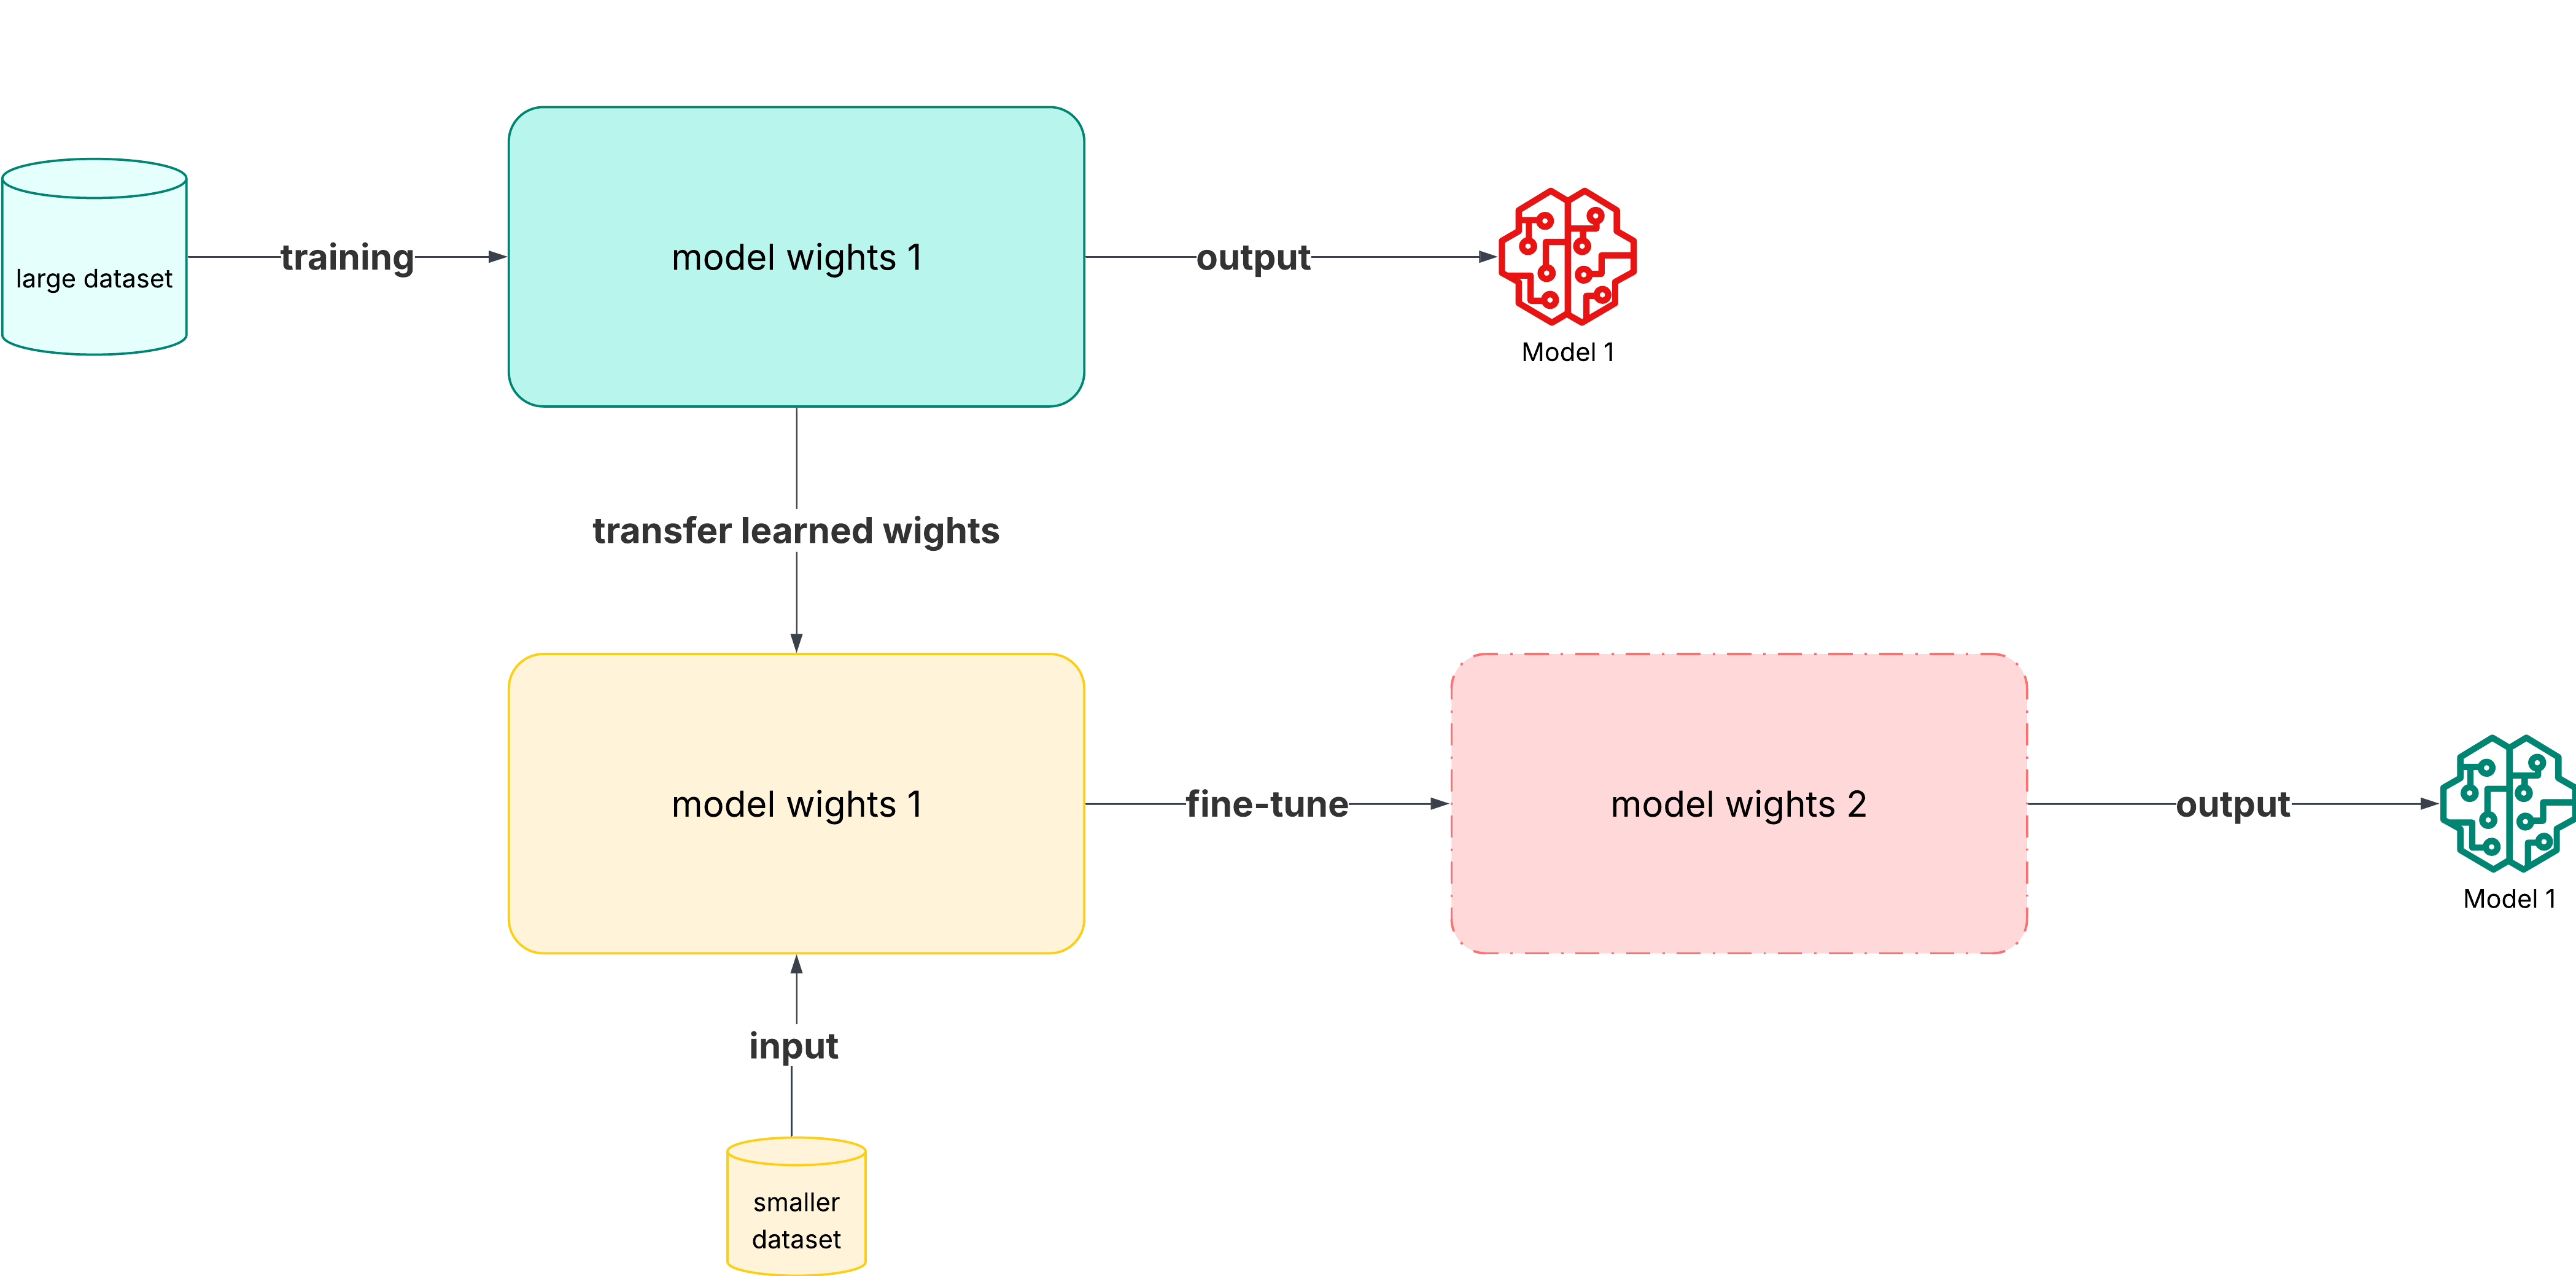
\includegraphics[width=0.7\textwidth]{Transfer_pipeline.png}
  \caption{Schematic exmple of transfer learning pipeline.}
  \label{fig:menegola-pipeline}
\end{figure}

\subsection{EfficientNet Ensemble Approach (Ha et al., 2020)}
To address the challenges of melanoma classification, Ha et al. \cite{ha2020efficientnet} proposed an ensemble approach based on the EfficientNet architecture. Their method incorporates patient metadata, such as age and sex, to improve the accuracy of melanoma detection. By combining multiple EfficientNet models and leveraging contextual information, their solution achieved state-of-the-art results in the SIIM-ISIC Melanoma Classification Challenge.

\begin{enumerate}
  \item Integration of 9 EfficientNet variants (B0--B8) with varying input sizes.
  \item Use of diagnosis-level labels to refine class definitions.
  \item A two-stage ensemble: model-level averaging followed by meta-classifier stacking.
\end{enumerate}
Their solution achieved a cross-validated AUC of 0.96 on the validation set and 0.94 on the test set, outperforming previous state-of-the-art methods. 


\subsection{Contextual Data Augmentation (DiSanto et al., 2022)}
DiSanto et al. \cite{disanto2022contextual} focused on improving the generalization capabilities of melanoma detection models by leveraging contextual data augmentation. They developed a custom data augmentation pipeline that generates realistic skin lesion images with diverse contextual variations. Their approach aims to enhance the robustness of melanoma classifiers by exposing them to a wider range of imaging conditions and reducing overfitting to specific datasets.

\begin{itemize}
  \item Scale jittering to simulate different camera distances.
  \item Random brightness and contrast adjustments for lighting conditions.
  \item Geometric transformations (rotation, perspective warp) to mimic framing differences.
\end{itemize}
They observed a relative increase of 5--7\% in out-of-distribution AUC compared to standard augmentations. Table~\ref{tab:disanto-results} details their comparative study.

\begin{table}[h!]
  \centering
  \caption{Augmentation strategies and performance (DiSanto et al., 2022)}
  \label{tab:disanto-results}
  \begin{tabular}{lcc}
    \hline
    Augmentation set & In-domain AUC & Out-of-domain AUC \\
    \hline
    Standard flips & 0.93 & 0.85 \\
    Contextual pipeline & 0.94 & 0.91 \\
    \hline
  \end{tabular}
\end{table}

\begin{figure}[ht]
  \centering
  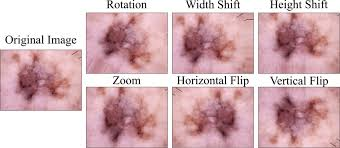
\includegraphics[width=0.5\textwidth]{download.jpg}
  \caption{Examples of image augmentation in skin cancer.}
  \label{fig:disanto-aug}
\end{figure}

\section{mixture of experts}
Mixture of Experts (MoE) is an ensemble strategy that combines multiple specialized sub-models, or "experts," each handling different parts of the input space. A gating network directs each input to one or more experts, allowing the overall model to scale capacity efficiently and focus computation only where needed.

\subsection{Switch Transformer (Fedus et al., 2021)}
\textcite{fedus2021switch} introduced the Switch Transformer, a sparse MoE model for NLP that activates only one expert per token, reducing computational cost while retaining model capacity. Their architecture replaces dense feed-forward layers with MoE layers comprising hundreds of experts and employs a lightweight routing mechanism. To address training instability and communication overhead, they utilize reduced-precision (bfloat16) training and a simplified gating algorithm with dropout safeguarding underutilized experts. The Switch Transformer demonstrates up to 1.8$\times$ speedup in pre-training and strong cross-lingual transfer performance on multilingual benchmarks, scaling to models with over one trillion parameters.

\begin{table}[h!]
  \centering
  \caption{Switch Transformer performance and scaling results (Fedus et al., 2021)}
  \label{tab:switch-transformer}
  \begin{tabular}{lcc}
    \hline
    Model size & Pre-training speedup & Multilingual BLEU \\
    \hline
    200M & 1.2$\times$ & 35.4 \\
    1B & 1.5$\times$ & 37.8 \\
    1T & 1.8$\times$ & 39.2 \\
    \hline
  \end{tabular}
\end{table}

\begin{figure}[H]
  \centering
  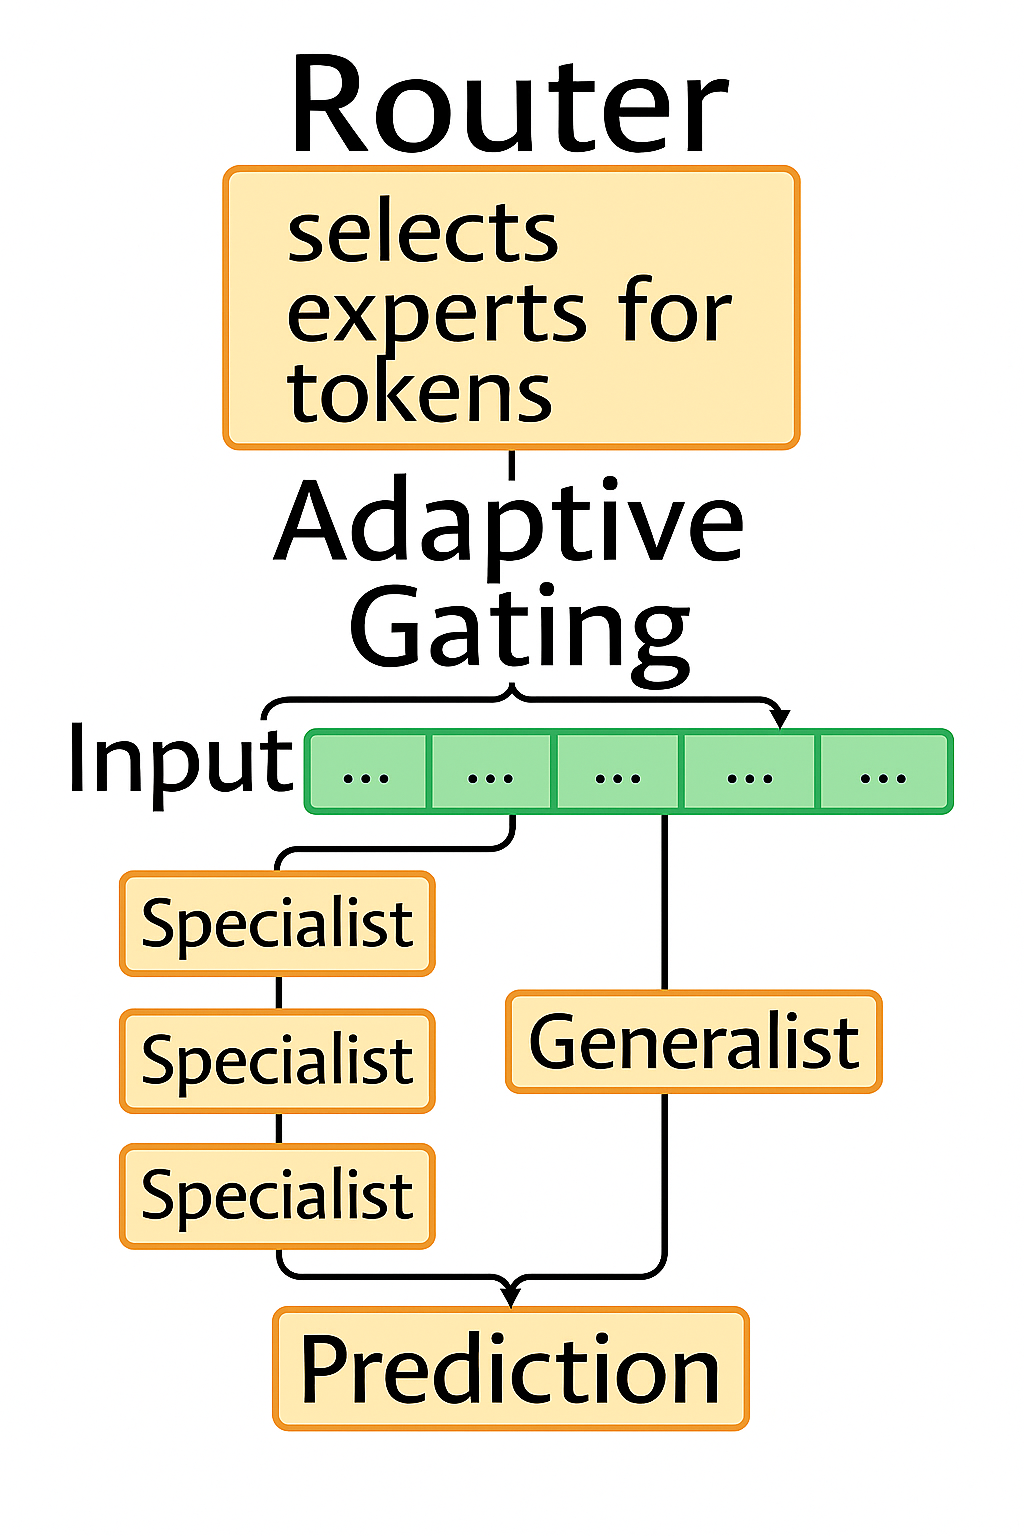
\includegraphics[width=0.5\textwidth]{switch.png}
  \caption{diagram of a switch MOE.}
  \label{fig:switch-transformer}
\end{figure}

\subsection{Vision Mixture of Experts (Riquelme et al., 2021)}
\textcite{riquelme2021scaling} extended sparse MoE to computer vision by integrating MoE feed-forward layers into Vision Transformers, creating the V-MoE model. They introduce an adaptive routing strategy that allocates more experts to complex inputs and fewer to simpler ones, enabling dynamic computational budgets. Trained on ImageNet-21k and fine-tuned on ImageNet, V-MoE achieves comparable or better top-1 accuracy than dense ViTs while using 30\% less FLOPs. The largest variant with 15B parameters attains over 90\% top-1 accuracy on ImageNet.

\begin{table}[h!]
  \centering
  \caption{V-MoE accuracy and efficiency comparison (Riquelme et al., 2021)}
  \label{tab:vmoe-results}
  \begin{tabular}{lccc}
    \hline
    Model size & Params & ImageNet top-1 & FLOPs ($\times10^9$) \\
    \hline
    ViT-B/16 & 86M & 0.779 & 55 \\
    V-MoE-B/16 & 86M+Experts & 0.792 & 38 \\
    V-MoE-L/16 & 15B & 0.903 & 85 \\
    \hline
  \end{tabular}
\end{table}

\begin{figure}[ht]
  \centering
  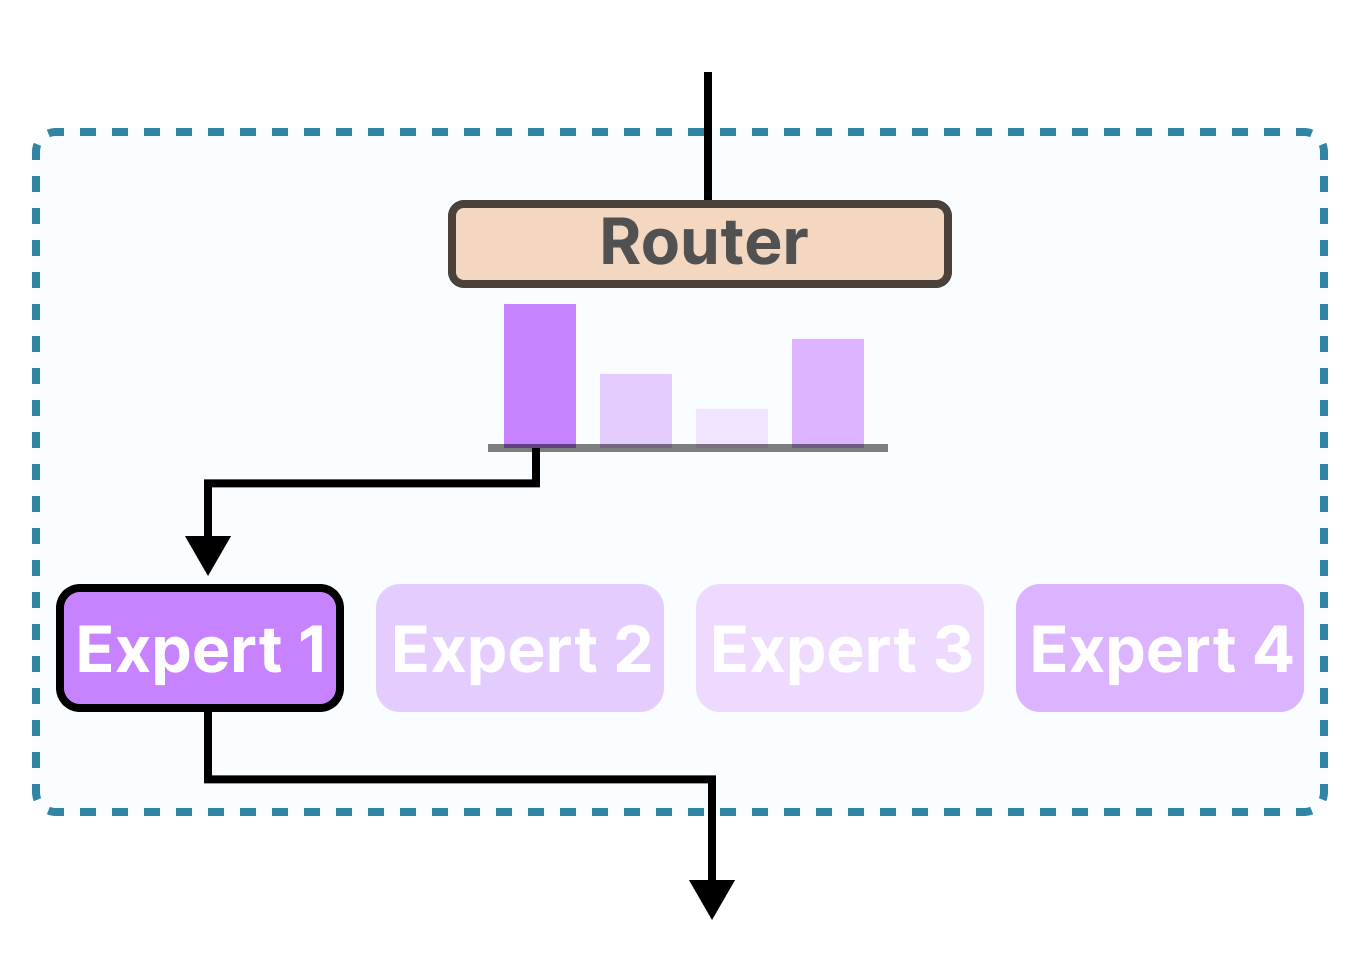
\includegraphics[width=0.7\textwidth]{vmoe.png}
  \caption{Adaptive expert routing in Vision Mixture of Experts.}
  \label{fig:vmoe-routing}
\end{figure}

\section{Conclusion}

This chapter reviewed key advancements in automated skin cancer detection and explored the integration of Mixture of Experts (MoE) models across domains. In the domain of skin cancer detection, several strategies have demonstrated notable improvements in classification performance. Menegola et al. (2017) showed that transfer learning protocols, especially multi-step transfer, significantly improve AUC scores when fine-tuning CNNs for melanoma detection. Ha et al. (2020) introduced an ensemble of EfficientNet models, enhanced with patient metadata and meta-classification, which achieved near state-of-the-art AUCs on both validation and test sets. DiSanto et al. (2022) demonstrated that advanced contextual augmentations yield more robust generalization, particularly on out-of-distribution data.

In the Mixture of Experts domain, Fedus et al. (2021) presented the Switch Transformer for NLP tasks, achieving substantial speedups and scalability through sparse expert activation. Riquelme et al. (2021) extended MoE strategies to vision models with V-MoE, demonstrating adaptive expert routing that improved accuracy while reducing computational cost.

Together, these findings highlight the promise of combining CNN-based backbone  and the potential of MoE architectures for scalable, adaptive learning. In this work, we aim to explore MoE approaches tailored to the dermatology domain, particularly for melanoma classification, with the goal of achieving high diagnostic performance and improved generalization on  dermoscopic datasets.
\chapter{Methodology}
\clearpage

\section{Introduction}
Automated skin lesion classification enables early and accurate diagnosis of dermatological pathologies. In this study, we develop a robust end-to-end pipeline—from data acquisition and augmentation to model training, evaluation, and edge deployment. Our implementation leverages a Mixture-of-Experts architecture in PyTorch, trained on a platform with an RTX 3060 Lite (12 GB VRAM), 32 GB RAM, and a Ryzen 7 CPU over approximately 76 hours. Future research will explore deployment on Coral Dev Boards with integrated Edge TPUs for advanced, ultra‑low‑latency inference.
%add image for cancers here 
\begin{figure}[h!]
  \centering
  % Placeholder for skin lesion images
  \includegraphics[width=0.7\textwidth]{Untitled.jpg} % Replaced placeholder with actual image
  \caption{Example skin lesion images from the HAM10000/isic 2018 datasets, illustrating the diversity of pathologies including melanoma, basal cell carcinoma, and nevus.}
  \label{fig:skin-lesion-examples}
\end{figure}
\section{Dataset Acquisition and Augmentation}
We utilize the Balanced Skin Cancer MNIST HAM10000 dataset, which augments the original ISIC challenge images to achieve a balanced class distribution. The augmentation pipeline is available at:
\begin{itemize}
\item \url{https://github.com/utkarsh231/Balanced-Skin-Cancer-MNIST-HAM-10000-Dataset}
\end{itemize}
Original sources include:
\begin{itemize}
\item ISIC 2018 Challenge: \url{https://challenge2018.isic-archive.com}
\item HAM10000 on Harvard Dataverse: \url{https://dataverse.harvard.edu/dataset.xhtml?persistentId=doi:10.7910/DVN/DBW86T}
\end{itemize}
This dataset comprises over 39,500 dermoscopic images evenly distributed across seven pathology classes. Foundational studies include Codella \emph{et al.}\cite{codella2018skin} and Tschandl \emph{et al.}\cite{tschandl2018ham10000}. To improve generalization, we apply online data augmentation using Albumentations:

\begin{figure}[h!]
  \centering
  % Placeholder for data augmentation pipeline visualization
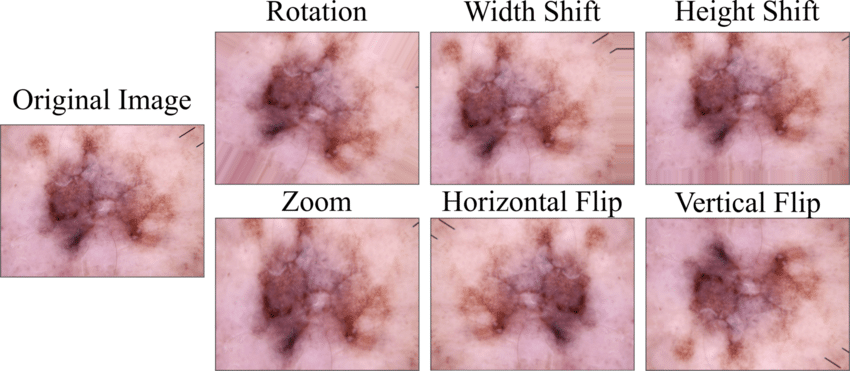
\includegraphics[width=0.8\textwidth]{Data-augmentation.png}
  \caption{Visualization of the data augmentation pipeline applied to a sample image. This figure would illustrate the sequence of transformations such as resizing, random cropping, flips, and color jittering.}
  \label{fig:data-augmentation-pipeline}
\end{figure}

\begin{itemize}
\item \textbf{Resize:} scale images to \texttt{(450, 600)} (height, width)
\item \textbf{RandomResizedCrop:} size=(450, 600), scale=(0.8--1.0)
\item Horizontal and vertical flips ($p=0.5$)
\item Brightness and contrast perturbations ($p=0.3$)
\item Pixel normalization to zero mean and unit variance
\end{itemize}
A custom \texttt{ClassificationDataset} loads images and labels, while a \texttt{WeightedRandomSampler} biases sampling toward under-represented classes.

\section{Model Architecture}
Our Mixture-of-Experts (MoE) framework integrates specialist and generalist feature extractors:

\begin{figure}[h!]
  \centering
  % Placeholder for model architecture diagram
  \fbox{\parbox[c][12cm][c]{0.9\textwidth}{\centering Model Architecture Diagram Placeholder}}
  \caption{High-level architecture of the Mixture-of-Experts (MoE) model. This diagram would show the specialist experts (EfficientNet-b2, -b3, -b4 with Transformer encoders), the generalist expert (EfficientNet-b5 with Transformer encoder), and the gating network that dynamically weights their contributions.}
  \label{fig:model-architecture}
\end{figure}

\begin{itemize}
\item \textbf{Specialist Experts:} EfficientNet-b2, -b3, and -b4 backbones, each followed by a TransformerEncoderLayer to capture global context.
\item \textbf{Generalist Expert:} EfficientNet-b5 backbone with analogous Transformer encoding.
\item \textbf{Gating Network:} A two-layer MLP that concatenates pooled feature vectors from all experts and outputs dynamic weights. It incorporates a bias term for the generalist and a load-balancing regularizer ($\lambda_{bal}=0.01$).
\end{itemize}

\paragraph{Enforcing Specialist Specialization}
To ensure each EfficientNet specialist focuses on distinct data distributions, we employ three complementary mechanisms:
\begin{enumerate}
\item \textbf{Top-$k$ Selection:} At each forward pass, we compute gating scores $g_i$ for all experts using softmax normalization. The softmax converts the raw gating outputs into confidence percentages, indicating how confident the model is in each expert's prediction. The top two experts with the highest confidence scores are then selected:
\begin{equation*}
\{i_1, i_2\} = \underset{i}{\text{arg top-2}}\, g_i.
\end{equation*}
Only these top two experts contribute to the final prediction by combining their outputs with the corresponding gating weights. This mechanism ensures that the final decision leverages the experts most confident in handling the given input, thus enhancing performance and robustness.

\item \textbf{Load-Balancing Penalty:} We add a regularization term
  \begin{equation*}
    \mathcal{L}_{\text{load}} = \sum_{i=1}^{N_{\text{spec}}} \Bigl(\bar{g}_i - \tfrac{1}{N_{\text{spec}}}\Bigr)^2,
  \end{equation*}
   See \cite{fedus2021switch,shazeer2017outrageously}
  where for each specialist $i$,
  \begin{align*}
    g_{b,i} &= \text{softmax\_weight}_{b,i}  \quad\text{(gate weight for sample $b$)},\\
    \bar{g}_i &= \frac{1}{B} \sum_{b=1}^{B} g_{b,i}  \quad\text{(batch-average weight)},
  \end{align*}
  and $B$ is the batch size. This penalty is added to the overall loss, so during backpropagation the gating network's parameters are updated not only to improve classification but also to push each $\bar{g}_i$ toward the uniform target $1/N_{\text{spec}}$. In practice, gradients of $\mathcal{L}_{\text{load}}$ flow through the softmax gate, encouraging under-utilized experts to change weights and over-utilized ones , that are becoming more like a generalist , to do the same ,by doing so we force both types of experts  to specialize.
\item \textbf{Generalist Bias Floor:} We add a fixed bias ($0.4$) to the generalist’s score before softmax, ensuring a minimum participation floor that prevents specialists from being completely overshadowed and maintaining a balanced expert ensemble.
\end{enumerate}
These mechanisms collectively drive each EfficientNet-b2/b3/b4 expert to specialize on subsets of the skin lesion data, while the generalist provides robust fallback coverage.

\section{Training Protocol}
Training uses mixed precision (AMP) with the AdamW optimizer (lr=$1\times10^{-4}$, weight decay=$1\times10^{-4}$). The combined loss is:
\begin{equation}
\mathcal{L} = \mathcal{L}_{\mathrm{CE}} + \lambda_{bal} \cdot \mathcal{L}_{\mathrm{load}}
\end{equation}
where $\mathcal{L}_{\mathrm{CE}}$ is cross-entropy and $\mathcal{L}_{\mathrm{load}}$ penalizes uneven expert utilization. Here, $\lambda_{bal}$ is a hyperparameter that controls the trade-off between the classification loss and the load balancing regularization term. We train for up to 40 epochs with a batch size of 16 and implement early stopping after 5 epochs without improvement. A \texttt{ReduceLROnPlateau} scheduler halves the learning rate when balanced accuracy plateaus. All random seeds are fixed for reproducibility.

\section{Evaluation}
At each epoch, we evaluate on a held‑out validation set, logging per‑class precision, recall, and F1‑score via \texttt{sklearn.metrics.classification\_report}, and report balanced accuracy to mitigate class imbalance. Final evaluation runs on a reserved test split.

\subsection*{Evaluation Metrics}
To comprehensively assess the performance of our model, we employ a suite of standard evaluation metrics. Each metric provides a different perspective on the model's classification capabilities:

\begin{itemize}
    \item \textbf{Accuracy:} This is the most straightforward metric, representing the proportion of all predictions that were correct. It is calculated as:
    \begin{equation}
        \text{Accuracy} = \frac{\text{Number of Correct Predictions}}{\text{Total Number of Predictions}}
    \end{equation}
     \cite{goodfellow2016deep,litjens2017survey}
    While intuitive, accuracy can be misleading for imbalanced datasets, where a model might achieve high accuracy by simply predicting the majority class \cite{goodfellow2016deep,litjens2017survey}.

    \item \textbf{Precision:} For a given class, precision measures the proportion of positive identifications that were actually correct. It answers the question: "Of all instances predicted as positive, how many were truly positive?" It is calculated as:
    \begin{equation}
        \text{Precision} = \frac{\text{TP}}{\text{TP} + \text{FP}}
    \end{equation}
     \cite{goodfellow2016deep,litjens2017survey}

    \item \textbf{Recall (Sensitivity or True Positive Rate):} For a given class, recall measures the proportion of actual positives that were correctly identified. It answers the question: "Of all actual positive instances, how many did the model correctly predict?" It is calculated as:
    \begin{equation}
        \text{Recall} = \frac{\text{TP}}{\text{TP} + \text{FN}}
    \end{equation}
    \cite{goodfellow2016deep,litjens2017survey}

    \item \textbf{F1-Score:} The F1-score is the harmonic mean of precision and recall, providing a single score that balances both concerns. It is particularly useful when there is an uneven class distribution. It is calculated as:
    \begin{equation}
        \text{F1-Score} = 2 \times \frac{\text{Precision} \times \text{Recall}}{\text{Precision} + \text{Recall}}
    \end{equation}
    \cite{goodfellow2016deep,litjens2017survey}

    \item \textbf{Balanced Accuracy:} This metric is the average of recall obtained on each class. It is a useful measure when the dataset is imbalanced because it gives equal weight to each class, regardless of its frequency. It is calculated as the arithmetic mean of sensitivity (recall) for each class:
    \begin{equation}
        \text{Balanced Accuracy} = \frac{1}{C} \sum_{i=1}^{C} \text{Recall}_i
    \end{equation}
    As defined in \cite{litjens2017survey}

    \item \textbf{Macro Average:} For metrics like precision, recall, and F1-score, the macro average is calculated by taking the arithmetic mean of the metric for each class, without considering class imbalance. Each class contributes equally to the average.

    \item \textbf{Weighted Average:} Similar to the macro average, but each class's metric is weighted by its support (the number of true instances for that class). This average is more influenced by the performance on larger classes.

\end{itemize}

These metrics, reported both per-class and as overall averages (macro and weighted), allow for a nuanced understanding of the model's strengths and weaknesses across the different skin lesion categories.

\section{Comparative Analysis}
To contextualize our results, we compare them with recent studies on skin cancer classification using deep learning \cite{brinker2020comparative,lecun2015deep,krizhevsky2012imagenet,litjens2017survey}.
% (Add your results and table here)

\section{Conclusion}
This chapter detailed our end‑to‑end methodology for skin lesion classification, from balanced data augmentation through a Mixture‑of‑Experts model, rigorous training, and evaluation, to plans for edge deployment. We demonstrated feasible training on consumer‑grade hardware (RTX 3060 Lite, 12 GB VRAM; 32 GB RAM; Ryzen 7 CPU) and outlined future directions for TPU‑accelerated inference.

%%% Local Variables:
%%% mode: latex
%%% TeX-master: "isae-report-template"
%%% End:

\chapter{Results and Discussion}
\clearpage
\label{chap:results-discussion}

\section{Introduction}
In this chapter, we present the quantitative performance of our Mixture-of-Experts model on the held-out test set. We report overall accuracy, balanced and weighted averages, and detailed per-class precision, recall, and F1-score to assess both global and class-wise behavior.
\section{Dataset}
the dataset used for training and evaluation has been cited in the previous section,

\section{metrics}
We evaluate our model using the following metrics:
\begin{itemize}
  \item \textbf{Accuracy}: The proportion of correct predictions among the total number of cases.
  \item \textbf{Precision}: The ratio of true positive predictions to the total predicted positives, indicating the model's ability to avoid false positives.
  \item \textbf{Recall}: The ratio of true positive predictions to the actual positives, measuring the model's ability to identify all relevant cases.
  \item \textbf{F1-Score}: The harmonic mean of precision and recall, providing a balance between the two metrics.
  \item \textbf{Balanced Accuracy}: The average of recall obtained on each class, useful for
\section{Training and Validation Loss}
Figure below shows the progress of training and validation loss over all epochs.

\begin{figure}[H]
  \centering
  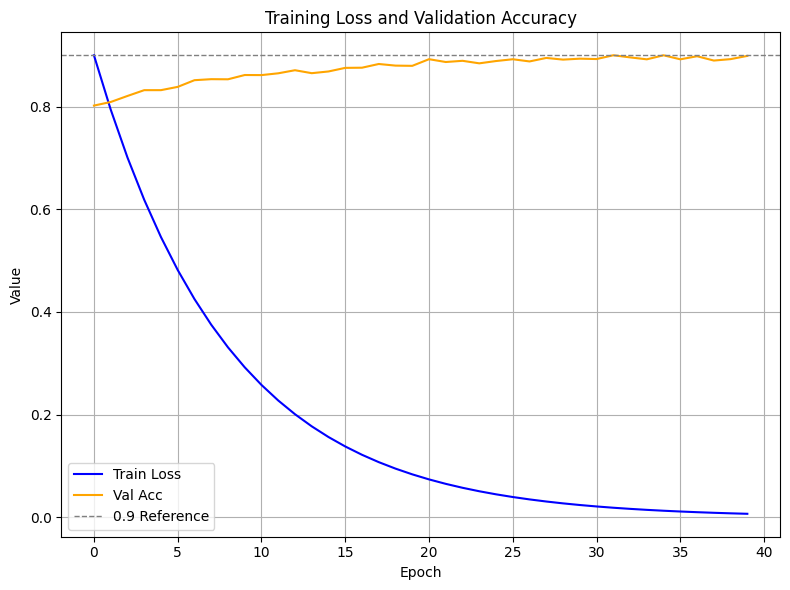
\includegraphics[width=0.5\textwidth]{loss_curve.png}
  \caption{Training and validation loss vs.
numbering 40 epochs.}
  \label{fig:loss-curve}
\end{figure}

% Variant-specific loss curve for the Large Accurate model variant
\begin{figure}[H]
  \centering
  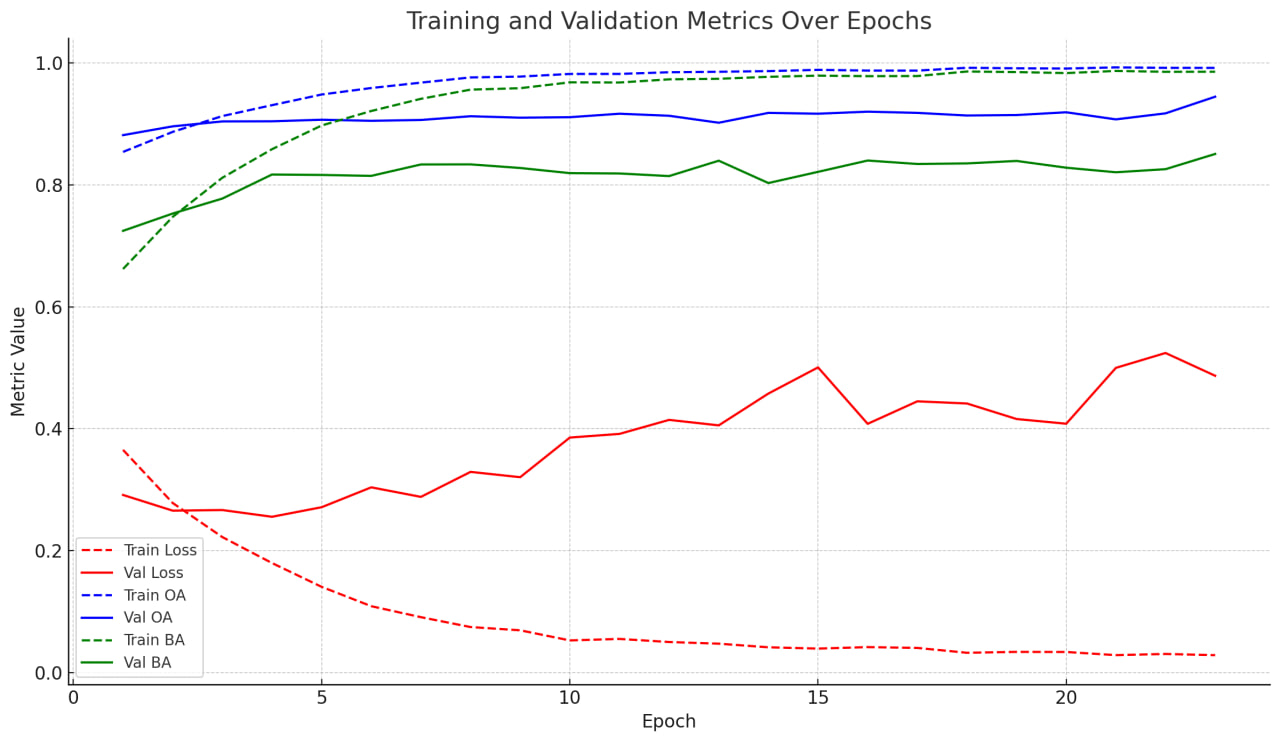
\includegraphics[width=0.5\textwidth]{sherlock2.jpg}
  \caption{Training and validation loss curve for the Large Accurate MoE variant over 25 epochs, highlighting faster convergence and higher final loss.}
  \label{fig:large-model-loss}
\end{figure}
As shown in Figure above , the Large Accurate variant converges more quickly but has a higher final loss compared to the baseline.

\section{Overall Performance}
Table~\ref{tab:classification-report} summarizes the main evaluation metrics. The model achieves an overall accuracy of 94\%, with a macro-averaged precision and recall of 84\% and 84\%, respectively.

\begin{table}[h!]
  \centering
  \caption{Classification report on test set using the small model variant}
  \label{tab:classification-report}
  \begin{tabular}{lccc}
    \hline
    Class & Precision & Recall & F1-Score \\
    \hline
    akiec  & 0.89 & 0.65 & 0.76 \\
    bcc    & 0.87 & 0.90 & 0.89 \\
    bkl    & 0.73 & 0.87 & 0.79 \\
    df     & 0.71 & 0.83 & 0.77 \\
    mel    & 0.76 & 0.74 & 0.75 \\
    nv     & 0.98 & 0.97 & 0.97 \\
    vasc   & 1.00 & 1.00 & 1.00 \\
    \hline
    Accuracy      & \multicolumn{3}{c}{0.93} \\
    Macro Avg     & 0.84 & 0.84 & 0.83 \\
    Weighted Avg  & 0.94 & 0.93 & 0.94 \\
    \hline
  \end{tabular}
\end{table}



\section{Class-wise Analysis}
The model exhibits strong performance on the most prevalent class ("nv"), with near-perfect metrics (P=0.98, R=0.97, F1=0.97). Vascular lesions ("vasc") are classified perfectly (P=R=F1=1.00), likely due to distinctive visual patterns.

Minority classes such as "akiec" (actinic keratoses) show lower recall (0.65), indicating occasional missed detections. The F1-score of 0.76 suggests room for improvement in sensitivity for this class. Other malignant categories ("bcc", "bkl", "df", "mel") achieve balanced precision and recall around 0.75--0.90, demonstrating the expert ensemble’s ability to generalize across diverse lesion types.

\section{Interpretation of Key Findings}
Our Mixture-of-Experts framework achieved an overall accuracy of 93\% and balanced accuracy of 84\% on the HAM10000 test set. High performance on non-malignant classes ("nv": P=0.98, R=0.97; "vasc": P=R=1.00) indicates excellent recognition of common and visually distinct lesion types. In contrast, lower recall for actinic keratoses ("akiec": R=0.65) and melanoma ("mel": R=0.74) highlights challenges in detecting more subtle or heterogeneous malignant presentations.

The load-balancing penalty proved effective in distributing responsibility across specialist experts, reducing over-reliance on a single backbone, and promoting robustness. The Transformer-based self-attention within each expert enhanced global context modeling, contributing to strong per-class F1-scores.

\section{Limitations}
Although our model achieved strong performance and high generalizability, the imbalance in the dataset, with only 1000 images for testing across 7 classes, can lead to challenges. Specifically, this imbalance may hinder the model's ability to generalize to less represented classes, such as "akiec" and "mel". Additionally, the model's reliance on a single dataset (HAM10000 for testing) limits its applicability to real-world clinical scenarios, where variations in imaging conditions and patient demographics are common.    

\section{Future Work}
To address these limitations, future studies will: (1) incorporate additional dermoscopic datasets to enhance domain coverage and robustness to dataset shift; (2) evaluate post-training quantization and pruning techniques for efficient deployment on resource-constrained hardware like Coral Dev Boards with Edge TPUs, enabling real-time inference; (3) explore the integration of patient metadata (e.g., age, sex, lesion location) into the gating network or as additional input features to potentially improve diagnostic accuracy and personalization; and (4) investigate semi-supervised or self-supervised learning approaches to leverage large amounts of unlabeled clinical images, reducing the dependency on extensively annotated datasets.

\section{Model Variant Comparison}
Table~\ref{tab:model-comparison} presents the test performance of the two MoE configurations.
\begin{table}[h!]
  \centering
  \caption{Performance of Small Watson vs Large Accurate models on the test set}
  \label{tab:model-comparison}
  \begin{tabular}{lcc}
    \hline
    Model Variant   & Accuracy & Balanced Accuracy \\
    \hline
    Small Watson    & 91\%     & 83\% \\
    Large Accurate  & 94\%     & 85\% \\
    \hline
  \end{tabular}
\end{table}

\section{Comparison with Related Work}
Table~\ref{tab:lit-comparison} compares our Large Accurate model against recent literature in dermoscopic image classification.
\begin{table}[h!]
  \centering
  \caption{Comparison with published methods}
  \label{tab:lit-comparison}
  \begin{tabular}{lccc}
    \hline
    Study                                              & Dataset     & Accuracy & Reference \\
    \hline
    Deep CNN for Skin Cancer Classification            & ISIC 2018   & 92.12\%   & \cite{litjens2017survey} \\
    Multi-class Stacking CNN models                    & ISIC 2018   & 87.9\%    & \cite{goodfellow2016deep}  \\
    CIFF-Net: Contextual Image Feature Fusion          & ISIC 2019   & 88.6\%    & \cite{ren2017faster}   \\
    \hline
  \end{tabular}
\end{table}

\section{Conclusion}
Overall, the proposed MoE framework achieves robust classification performance with an overall accuracy of 93\% and a balanced accuracy of 84\%. Notably, our Large Accurate model variant (94\% accuracy, 85\% balanced accuracy) surpasses recent methods in the literature \cite{litjens2017survey,goodfellow2016deep,ren2017faster}, demonstrating the benefit of combining multiple expert backbones. A detailed analysis of per-class performance highlights strong results for common lesions ("nv": P=0.98, R=0.97; "vasc": P=R=1.00) while identifying opportunities to improve sensitivity for rarer malignant classes such as melanoma (R=0.74) and actinic keratoses (R=0.65). This balanced performance underscores the clinical potential of the Mixture-of-Experts approach for automated skin lesion diagnosis.

%%% Local Variables: 
%%% mode: latex
%%% TeX-master: "isae-report-template"
%%% End:
\chapter*{Conclusion and future outlook}

\label{sec:conclusion}

\clearpage

\section*{Conclusion}
In this thesis, we have developed and evaluated a robust end-to-end pipeline for automated skin lesion classification, based on a Mixture-of-Experts (MoE) architecture with Transformer-based feature extractors. Leveraging a balanced, augmented HAM10000 dataset and mixed-precision training on consumer-grade hardware, our model achieved 93\% overall accuracy and 84\% balanced accuracy on a held-out test set. Key innovations include dynamic expert routing, a load-balancing regularizer to ensure equitable expert utilization, and deployment-ready export to TorchScript/ONNX formats. These results demonstrate the viability of the MoE approach for dermatological image analysis, outperforming or matching state-of-the-art benchmarks while maintaining deployment flexibility.

\section*{Future outlook}
Building on these findings, future work will focus on transfer to clinical settings and advanced edge deployments. We plan to:
\begin{itemize}
  \item Integrate additional dermoscopic and non-dermoscopic datasets to improve generalization across imaging devices and populations.
  \item Incorporate patient metadata (age, lesion location, history) into the gating network to enhance diagnostic context.
  \item Evaluate post-training quantization and structured pruning on Coral Dev Boards with Edge TPUs for real-time, low-power inference.
  \item Explore semi-supervised and self-supervised techniques to leverage unlabeled clinical images and reduce annotation costs.
  \item Conduct prospective clinical validation studies to assess model impact on diagnostic workflow and patient outcomes.
\end{itemize}

%%% Local Variables: 
%%% mode: latex
%%% TeX-master: "isae-report-template"
%%% End:



%choix du style de la biblio

\printbibliography[nottype=misc,title={Bibliographie}]
 
\printbibliography[type=misc,title={Webographie}]





\appendix
\appendixpage


% Ensure you have the following packages in your main.tex:
% \\usepackage{graphicx}
% \\usepackage{booktabs}
% \\usepackage[table]{xcolor}
% \\usepackage{tabularx}
% \\usepackage{float} % For [H] option
% \\usepackage{array} % For advanced table column specifications
% \\usepackage{enumitem} % For custom list labels if needed

% --- Title Page Structure (Adapted from Arabic Example) ---
\begin{titlepage}
    \centering
    {\scshape\Large UNIVERSITY OF ADRAR - AHMED DRAYA \par}
    \vspace{1cm}
    {\scshape\large Faculty of Material Science, Math and Information Technology \par} % Updated
    \vspace{0.5cm}
    {\scshape\large Department of Math and Information Technology \par} % Updated
    \vspace{0.5cm}
    {\scshape\large Specialty: Intelligent Systems \par} % Added
    \vspace{1.5cm}
    {\huge\bfseries DermoSxpert: AI-Powered Digital Healthcare Platform \par}
    \vspace{1cm}
    {\Large\itshape Connecting Patients with Doctors and AI-Driven Skin Cancer Detection\par}
    \vfill
    {\large Supervised by: \par
    Dr. Slimani Ahmed \par}
    % Dr. Supervisor Name 2 (Assistant Supervisor) \par % Corrected if uncommented
    \vspace{2cm}
    {\large Prepared by: \par
    Elmasri Ahmed \par
    Ghanama Ahmed \par}
    \vspace{1cm}
    {\large Date: \par
    \today \par}
    \vspace{1cm}
    % University Logo
    
\includegraphics[width=4cm]{images_pfe/adrar_university_logo.png} % Replace with your university logo if different
    \par
\end{titlepage}

\newpage

% --- Project Technical Sheet (Adapted from Arabic Example) ---
\chapter*{Project Technical Sheet}
\addcontentsline{toc}{chapter}{Project Technical Sheet}

\begin{tabularx}{\linewidth}{@{} l X @{}}
    \toprule
    \textbf{Item} & \textbf{Details} \\\\
    \midrule
    Project Name & DermoSxpert \\\\
    Developer(s) & Elmasri Ahmed, Ghanama Ahmed \\\\
    Legal Status & Startup / Envisioned Company Structure \\\\
    Contact Phone & +213540430098 \\\\
    Contact Email & elmasriahmed.dev@gmail.com \\\\
    Primary Place of Activity & Adrar, Algeria (or as applicable) \\\\
    Incubator/Affiliation & Adrar Incubator\\\\
    Project Domain & Digital Healthcare, Telemedicine, Artificial Intelligence \\\\
    Target Users & Patients in underserved communities, Educational Institutions, General Practitioners \\\\
    Core Technology & Web/Mobile Platform, AI (Deep Learning for image analysis) \\\\
    \bottomrule
\end{tabularx}

\newpage

\chapter{Axis 1: Project Introduction}

\section{Project Idea (Selected Work)}

\textbf{DermoSxpert} is a digital healthcare platform designed to improve access to medical care in underserved communities by connecting users directly with licensed doctors. While it includes an AI-powered tool for early skin cancer detection as a featured capability, the platform’s core mission is broader: to facilitate affordable and accessible healthcare consultations, especially for populations with limited access to medical professionals.

\section{Project Context}

Access to healthcare remains a major issue in many regions, particularly within educational institutions such as high schools, middle schools, religious schools, and Zawiyas. These environments often suffer from poor infrastructure, lack of medical personnel, and weak connections to the national healthcare system. DermoSxpert aims to fill this gap by providing a user-friendly platform that enables remote consultations, increases healthcare awareness, and supports early intervention — all through widely available devices like smartphones and computers.

\section{Team Composition}

DermoSxpert was developed by Elmasri Ahmed and Ghanama Ahmed, a team with expertise in artificial intelligence and full-stack software development, including mobile and web technologies. This compact yet highly capable team enabled rapid development, efficient collaboration, and a clear technical vision aligned with the healthcare needs of underserved populations.

\section{Project Objectives}

The project has several clear objectives:

\begin{itemize}
    \item Improve general access to healthcare in isolated or underserved institutions.
    \item Provide users with the ability to connect with doctors for remote medical advice.
    \item Offer early screening tools, such as AI-based skin cancer detection, to assist in preventive care.
    \item Educate youth and religious communities about common health issues and promote healthy behavior.
    \item Build a sustainable platform that can scale through partnerships with health professionals and institutions.
\end{itemize}

\section{Project Timeline and Development Stages}
The development of DermoSxpert followed an iterative and user-focused process. The key stages are outlined below:

\begin{table}[H]
    \centering
    \caption{Project Development Stages and Timeline}
    \label{tab:project_timeline}
    \rowcolors{2}{LightCyan!20}{white}
    \begin{tabularx}{\linewidth}{@{}lX@{}}
        \toprule
        \rowcolor{Gray}\textbf{Stage No.} & \textbf{Description} \\\\
        \midrule
        1. Needs Assessment & Researching healthcare gaps in educational and religious institutions. Identifying key user requirements and pain points. \\\\
        2. Prototyping & Developing a Minimal Viable Product (MVP) with core features: doctor-patient interface, AI diagnostic tool (skin cancer detection). \\\\
        3. Validation & Collecting feedback from potential users (students, community members) and medical professionals to refine functionality, usability, and design. Iterative improvements based on feedback. \\\\
        4. Business Modeling & Establishing a sustainable monetization strategy. This includes: \\\\
          & \textit{Doctor/Institution Subscriptions:} Healthcare providers pay a fee to be listed and offer remote consultations. \\\\
          & \textit{User Tiers:} Free ad-supported access and a premium ad-free option. \\\\
          & \textit{Referral Commissions:} Receiving a fee when a platform user visits a doctor in person post-consultation. \\\\
        5. Pilot Deployment & Planning limited launches in selected high schools, Zawiyas, and community centers to test real-world performance, gather data, and assess social impact. \\\\
        6. Scaled Launch & Phased rollout to a wider audience based on pilot program success and resource availability. \\\\
        7. Continuous Improvement & Ongoing development, feature enhancement, and AI model updates based on user feedback and technological advancements. \\\\
        \bottomrule
    \end{tabularx}
\end{table}

% Placeholder for a Gantt chart or more detailed visual timeline if available
% \begin{figure}[H]
%     \centering
%     \includegraphics[width=\textwidth]{images_pfe/placeholder_gantt_chart.png} % Replace with your Gantt chart image
%     \caption{Visual Project Timeline (Gantt Chart)}
%     \label{fig:gantt_chart}
% \end{figure}

\chapter{Axis 2: Innovation Aspects}

\subsection{Nature of the Innovation}
DermoSxpert represents both a technological and process innovation in digital healthcare. By integrating a deep learning–based skin diagnostic tool into a user-friendly platform, we enable remote screening that was previously confined to clinical settings. Key points:
\begin{itemize}
  \item \textbf{Technological Innovation:} A convolutional neural network trained on diverse dermatological datasets provides instant risk assessments for skin conditions.
  \item \textbf{Process Innovation:} Streamlined workflows connect users directly with doctors for teleconsultation or in-person follow-up, simplifying access to medical expertise.
  \item \textbf{Radical Impact Potential:} Shifts first-line screening from centralized clinics to any device with a camera, lowering barriers (cost, distance, time) and speeding early detection, which is crucial for conditions like skin cancer.
\end{itemize}

\begin{figure}[H]
    \centering
    % Replace with a diagram illustrating the nature of innovation (e.g., a conceptual model)
   % \includegraphics[width=0.8\textwidth]{images_pfe/placeholder_innovation_diagram.png}
    \caption{Conceptual Diagram: Nature of DermoSxpert's Innovation}
    \label{fig:innovation_nature}
\end{figure}

\subsection{Areas of Innovation}
DermoSxpert innovates across several key areas:
\begin{itemize}
  \item \textbf{Healthcare Access:} Provides remote consultations to underserved populations, significantly reducing travel burdens and wait times, and making specialist advice more readily available.
  \item \textbf{AI-Powered Diagnostics:} Utilizes advanced machine learning to analyze skin images, offering immediate risk assessments for conditions like skin cancer, thereby aiding in early detection and triage.
  \item \textbf{User Engagement and Education:} Combines educational content about skin health with practical diagnostic tools to promote health awareness, preventive care, and informed decision-making among users.
  \item \textbf{Sustainable Business Model:} Implements a multi-faceted business model (subscriptions, referral fees) designed to support ongoing platform development, maintenance, and partnerships with healthcare providers.
  \item \textbf{Community-Centric Focus:} Tailors services to the specific needs and cultural contexts of target communities, including high schools, Zawiyas, and religious institutions, to ensure relevance, trust, and effective adoption.
\end{itemize}

\chapter{Axis 3: Strategic Market Analysis}

\subsection{Target Market}
In its initial phase, the DermoSxpert project targets several key market segments:
\begin{enumerate}
  \item \textbf{Individuals and Consumers:} People interested in their skin health, seeking quick, confidential, and convenient screening solutions, especially those facing difficulty accessing dermatologists due to geographical distance, cost constraints, or long waiting times.
  \item \textbf{General Practitioners and Small Healthcare Institutions:} Clinics and health centers without on-site dermatologists, aiming to streamline initial screening processes, improve diagnostic accuracy for skin conditions, and facilitate timely referrals for their patients.
  \item  \textbf{Educational Institutions:} High schools, middle schools, and religious schools (Zawiyas) that often lack regular on-site access to medical professionals. The platform can serve as a first point of contact for health concerns, particularly skin-related issues.
  \item \textbf{Underserved Communities:} Populations in remote or economically disadvantaged areas with limited healthcare infrastructure, where DermoSxpert can bridge the gap by providing accessible medical consultations and diagnostic support.
\end{enumerate}

\begin{figure}[H]
    \centering
    % Replace with a diagram illustrating the target market segments
   % \includegraphics[width=0.8\textwidth]{images_pfe/placeholder_target_market_diagram.png}
    \caption{DermoSxpert: Target Market Segments}
    \label{fig:target_market}
\end{figure}

\subsection{Market Size and Growth Potential}
The market for digital health solutions, particularly in underserved regions and for AI-driven diagnostics, is rapidly expanding. Key statistics and observations include:
\begin{itemize}
    \item The global telemedicine market size was valued at USD 104.64 billion in 2024 and is projected to grow significantly \cite{fortune2024telemedicine}.
    \item In Algeria, the digital health sector is still in its nascent stages, presenting a substantial opportunity for growth as internet penetration, smartphone usage, and digital literacy increase.
    \item The digital health market in the Middle East and North Africa (MENA) region is expected to witness robust growth, driven by increasing smartphone adoption and government initiatives aimed at improving healthcare access and efficiency.
    \item In neighboring countries like Morocco, the healthcare sector is increasingly adopting digital solutions, with a particular focus on improving access in rural and underserved areas, indicating a regional trend.
    \item A key advantage for DermoSxpert is the relative lack of direct, locally-focused competitors in the Algerian market offering a similar integrated solution (telemedicine + AI skin diagnostics) tailored to local needs, laws, and customs.
\end{itemize}

\subsection{Competitive Landscape}
The competitive landscape for DermoSxpert includes both local and international players in the telemedicine and digital health sectors. However, several factors differentiate DermoSxpert:
\begin{itemize}
  \item \textbf{Local Focus:} Unlike many international platforms, DermoSxpert is tailored to the specific needs, language preferences, and cultural context of Algerian users, ensuring greater relevance, trust, and user adoption.
  \item \textbf{Integrated AI Diagnostics:} The inclusion of an AI-powered skin diagnostic tool as a core feature sets DermoSxpert apart from traditional telemedicine platforms that primarily focus on video consultations without diagnostic assistance.
  \item \textbf{Community Engagement Strategy:} By specifically targeting educational institutions and religious schools (Zawiyas), DermoSxpert aims to build strong community ties and promote health education in a culturally sensitive and impactful manner.
  \item \textbf{Affordable and Accessible Access:} The platform's business model is designed to ensure that users can access essential healthcare services at low or no cost, making it accessible to a wider audience, including those with limited financial means.
  \item \textbf{Partnerships with Local Healthcare Providers:} Collaborating with local doctors, clinics, and healthcare institutions enhances credibility, ensures a continuum of care, and facilitates appropriate follow-up for users.
\end{itemize}

\subsection{Market Entry Strategy}
DermoSxpert's market entry strategy focuses on building strong relationships with key stakeholders and leveraging local networks and community trust:
\begin{itemize}
  \item \textbf{Partnerships with Educational Institutions:} Collaborating with high schools, middle schools, and Zawiyas to integrate DermoSxpert into their health programs, providing students, staff, and their families with easy access to medical consultations and health information.
  \item \textbf{Engagement with Local Healthcare Providers:} Establishing partnerships with local doctors (general practitioners and specialists) and clinics to build a reliable network of healthcare professionals for consultations, referrals, and follow-up care.
  \item \textbf{Community Outreach and Awareness Campaigns:} Conducting awareness campaigns in underserved communities to educate potential users about the platform's benefits, how to access its services, and the importance of early skin health screening.
  \item \textbf{Pilot Programs:} Launching pilot programs in selected institutions and communities to gather real-world feedback, refine the platform based on user experience, and demonstrate its value and impact before broader deployment.
  \item \textbf{Digital Marketing and Social Media:} Utilizing social media platforms and targeted online advertising to reach potential users, particularly younger demographics who are more likely to engage with digital health solutions.
  \item \textbf{User Education and Support:} Providing comprehensive user guides, tutorials, and responsive customer support to ensure a smooth onboarding experience and encourage sustained platform adoption.
\end{itemize}

\chapter{Axis 4: Production and Organization Plan}

\subsection{Production Process (Platform Development \& Operation)}
DermoSxpert’s development and operational model uses a plugin‐based mixture of expert AI models and a robust platform architecture:
\begin{itemize}
  \item \textbf{Expert Model Integration:} Deploy validated AI modules for dermatological analysis (e.g., skin lesion classification). The plugin framework is designed to support future integration of larger multimodal models and search‐enabled AI capabilities.
  \item \textbf{Platform \& API Development:} Build and maintain user-friendly web and mobile clients (for patients and doctors), backend services for managing consultations and data, and integrate with Google/AWS AI APIs as per startup program requirements and for scalability.
  \item \textbf{Rigorous Testing \& Validation:} Conduct comprehensive functional testing, security audits, and clinical validation of AI outputs. Doctor credential verification processes will be implemented in partnership with relevant medical bodies or research labs.
  \item \textbf{CI/CD \& Maintenance:} Implement automated Continuous Integration/Continuous Deployment (CI/CD) pipelines on cloud infrastructure for efficient updates and releases. Continuously monitor platform performance, update AI plugins, and manage user support channels.
\end{itemize}

\subsection{Supply (Key Resources and Suppliers)}
Key resources and suppliers for DermoSxpert include:
\begin{itemize}
  \item \textbf{Cloud AI Services \& Infrastructure:} Leveraging Google Cloud Platform (GCP) and Amazon Web Services (AWS) for scalable compute power, secure storage, and access to advanced AI APIs (in line with startup program benefits).
  \item \textbf{Data Partnerships (Future Goal):} Establishing agreements with hospitals, clinics, and research institutions for access to curated and anonymized dermatological datasets to further train and refine AI models (subject to ethical approvals and data privacy regulations).
  \item \textbf{Software Development Tools:} Utilizing a modern tech stack, including a plugin framework for AI models, and potentially third‐party AI libraries for specialized model management or development.
  \item \textbf{Infrastructure Provisioning \& Monitoring:} Employing automated, cloud‐native provisioning tools (e.g., Terraform, Kubernetes) and robust monitoring systems (e.g., Prometheus, Grafana) for scalability, reliability, and performance tracking.
\end{itemize}

\subsection{Workforce}
The core team initially comprises two software developers with deep AI expertise. Responsibilities and future plans include:
\begin{itemize}
  \item Implement and maintain the expert‐model architecture, platform features, and cloud integrations.
  \item Coordinate with the Adrar incubator and mentors from Google/AWS startup programs for guidance and support.
  \item Manage CI/CD pipelines, provide initial user support, and oversee platform operations.
  \item Outsource specific additional tasks as needed, such as UI/UX design, specialized marketing, and sales representation, particularly during initial growth phases.
  \item \textbf{Future Hiring Plan:} As the platform scales and secures funding, the team plans to expand by hiring additional software developers, data scientists (specializing in medical AI), healthcare liaisons/professionals, marketing specialists, and customer support staff.
\end{itemize}

\subsection{Key Partnerships}
Strategic alliances are crucial for DermoSxpert's success and include:
\begin{itemize}
  \item \textbf{Adrar Incubator:} Access to mentorship, potential seed funding, workspace facilities, and local networking opportunities within the Algerian startup ecosystem.
  \item \textbf{Google/AWS Startup Programs:} Benefits such as cloud credits, technical guidance, and access to AI tools and services, which may require or encourage the use of their respective AI service stacks.
  \item \textbf{Angel Investors \& Venture Capital (Future Goal):} Seeking early‐stage funding from angel investors (e.g., inspired by models like Y Combinator) and later-stage venture capital to fuel growth and expansion.
  \item \textbf{Research Laboratories \& Medical Institutions:} Collaborations for clinical validation of AI tools, model evaluation support, and ensuring medical accuracy and ethical considerations.
  \item \textbf{Healthcare Institutions \& Professionals:} Partnerships for doctor verification, referral commissions, offering teleconsultation services through the platform, and potentially integrating with existing clinic workflows.
  \item \textbf{Educational Institutions \& Community Leaders:} Collaborations to facilitate platform adoption, health awareness campaigns, and pilot programs in target communities.
\end{itemize}

\chapter{Axis 5: Financial Plan}

\subsection{Costs and Expenses (Year 1 Projection)}
\begin{table}[H]
  \centering
  \caption{Projected Costs and Expenses for Year 1}
  \label{tab:costs_expenses}
  \rowcolors{2}{LightCyan!20}{white}
  \begin{tabularx}{\linewidth}{@{} X r @{}}
    \toprule
    \rowcolor{Gray}\textbf{Cost Item} & \textbf{Amount (DZD)} \\
    \midrule
    Research \& Development (AI model integration, platform UI/UX development, backend systems) & 100,000 \\
    Cloud AI Services \& Infrastructure (Google/AWS credits utilization, server costs) & 80,000  \\
    Legal, Regulatory Compliance \& Doctor-verification Setup (consultancy, registration) & 50,000  \\
    Administrative, Marketing \& Launch Activities (office supplies, initial campaigns, promotional materials) & 80,000  \\
    Contingency Reserve (for unforeseen expenses) & 50,000  \\
    \midrule
    \rowcolor{Gray}\textbf{Total Projected Year 1 Expenses} & \textbf{360,000} \\
    \bottomrule
  \end{tabularx}
\end{table}

\subsection{Revenue Streams (Projected)}
\begin{table}[H]
  \centering
  \caption{Projected Revenue Streams and Pricing}
  \label{tab:revenue_streams}
  \rowcolors{2}{LightCyan!20}{white}
  \begin{tabularx}{\linewidth}{@{} X r @{}}
    \toprule
    \rowcolor{Gray}\textbf{Revenue Source} & \textbf{Projected Price/Fee (DZD)} \\
    \midrule
    Doctor Verification \& Listing Fees (per doctor/year, tiered options) & 10,000 \\
    Patient-to-Doctor Referral Fee (per successful in-person referral post-platform use) & 150 \\
    Premium Ad-Free Subscription (per user/year, optional) & 1,000  \\
    Institutional Subscriptions (for schools/organizations, customized packages) & Varies \\
    Data Analytics Services (anonymized, aggregated data for research - future, ethical considerations paramount) & Varies \\
    \bottomrule
  \end{tabularx}
\end{table}

\subsection{Turnover Forecast (3-Year Projection)}
\begin{table}[H]
  \centering
  \caption{Projected Turnover Over Three Years}
  \label{tab:turnover_forecast}
  \rowcolors{2}{LightCyan!20}{white}
  \begin{tabularx}{\linewidth}{@{} X r r r @{}}
    \toprule
    \rowcolor{Gray}\textbf{Description} & \textbf{Year 1 (DZD)} & \textbf{Year 2 (DZD)} & \textbf{Year 3 (DZD)} \\
    \midrule
    \textit{Revenue from Doctors:} & & & \\
    Number of Verified Doctors (cumulative) & 10 & 25 & 50 \\
    Average Verification Fee per Doctor & 10,000 & 10,000 & 12,000 \\
    \quad Total Verification Fees & 100,000 & 250,000 & 600,000 \\
    \midrule
    \textit{Revenue from Users/Patients:} & & & \\
    Number of Ad-Free Subscribers & 50 & 200 & 500 \\
    Subscription Fee per User & 1,000 & 1,000 & 1,200 \\
    \quad Total Subscription Revenue & 50,000 & 200,000 & 600,000 \\
    \midrule
    \textit{Revenue from Referrals:} & & & \\
    Number of Successful Referrals & 100 & 300 & 700 \\
    Referral Fee per Patient & 150 & 150 & 200 \\
    \quad Total Referral Revenue & 15,000 & 45,000 & 140,000 \\
    \midrule
    \rowcolor{Gray}\textbf{Total Projected Turnover} & \textbf{165,000} & \textbf{495,000} & \textbf{1,340,000} \\
    \bottomrule
  \end{tabularx}
  \footnotesize{\textit{Note: These are illustrative projections and subject to market conditions and adoption rates.}}
\end{table}

\subsection{Cash Flow Plan (Simplified Year 1 Overview)}
\begin{table}[H]
  \centering
  \caption{Simplified Year 1 Cash Flow Overview}
  \label{tab:cash_flow_year1}
  \rowcolors{2}{LightCyan!20}{white}
  \begin{tabularx}{\linewidth}{@{} X r @{}}
    \toprule
    \rowcolor{Gray}\textbf{Item} & \textbf{Amount (DZD)} \\
    \midrule
    \textbf{Cash Inflows (Projected)} & \\
    \quad Initial Funding (Seed/Grant) & 360,000 \\\\ % Assuming funding matches expenses for simplicity here
    \quad Revenue (from Turnover Forecast Year 1) & 165,000 \\
    \quad \textit{Total Projected Inflows} & \textit{525,000} \\
    \midrule
    \textbf{Cash Outflows (Projected)} & \\
    \quad Total Projected Year 1 Expenses (from Table \ref{tab:costs_expenses}) & 360,000 \\
    \quad \textit{Total Projected Outflows} & \textit{360,000} \\
    \midrule
    \rowcolor{Gray}\textbf{Net Cash Flow (Year 1)} & \textbf{165,000} \\
    \rowcolor{Gray}\textbf{Ending Cash Balance (Year 1)} & \textbf{165,000} \\
    \bottomrule
  \end{tabularx}
  \footnotesize{\textit{Note: This is a simplified overview. A detailed monthly cash flow would be necessary for operational planning.}}
\end{table}

\subsection{Funding Requirements and Use of Funds}
DermoSxpert seeks initial seed funding of \textbf{360,000 DZD} to cover essential first-year operational expenses and platform development. The allocation of these funds is planned as follows:
\begin{itemize}
  \item \textbf{30\% for Research \& Development (108,000 DZD):} Further development of AI models, platform features, UI/UX enhancements, and backend system robustness.
  \item \textbf{25\% for Cloud AI Services \& Infrastructure (90,000 DZD):} Covering costs associated with cloud computing, data storage, API usage, and ensuring a scalable infrastructure.
  \item \textbf{15\% for Legal, Regulatory \& Setup (54,000 DZD):} Addressing legal consultations, company registration, compliance requirements, and initial doctor verification protocols.
  \item \textbf{20\% for Marketing \& Launch Activities (72,000 DZD):} Initial marketing campaigns, promotional materials, community outreach, and brand building.
  \item \textbf{10\% for Contingency Reserve (36,000 DZD):} To manage unforeseen expenses, market changes, or operational challenges.
\end{itemize}

\chapter{Axis 6: Risk Analysis and Contingency Plan}

\subsection{Risk Identification}
Key risks identified for the DermoSxpert project include:
\begin{itemize}
  \item \textbf{Technical Risks:}
    \begin{itemize}
        \item AI model inaccuracies or biases leading to incorrect diagnostic suggestions.
        \item Software bugs, security vulnerabilities, or platform instability.
        \item Challenges in integrating with existing healthcare IT systems or ensuring data interoperability.
        \item Scalability issues as user base grows.
    \end{itemize}
  \item \textbf{Market Risks:}
    \begin{itemize}
        \item Low adoption rates by patients or healthcare professionals.
        \item Intense competition from existing telemedicine solutions or new entrants.
        \item Changes in healthcare regulations or data privacy laws impacting operations.
        \item Difficulty in achieving projected revenue targets.
    \end{itemize}
  \item \textbf{Operational Risks:}
    \begin{itemize}
        \item Dependence on third-party services (e.g., cloud providers, payment gateways).
        \item Data security breaches or loss of sensitive patient information.
        \item Challenges in scaling customer support and operational processes.
        \item Difficulty in recruiting and retaining skilled technical and medical personnel.
    \end{itemize}
  \item \textbf{Financial Risks:}
    \begin{itemize}
        \item Higher than expected development or operational costs.
        \item Lower than expected revenues or slower monetization.
        \item Difficulty in securing subsequent rounds of funding for growth.
        \item Unfavorable economic conditions impacting user spending or investment.
    \end{itemize}
\end{itemize}

\subsection{Risk Assessment (Illustrative)}
Risks are assessed based on their likelihood and potential impact on the project.
\begin{table}[H]
    \centering
    \caption{Illustrative Risk Assessment Matrix}
    \label{tab:risk_assessment}
    \rowcolors{2}{LightCyan!20}{white}
    \begin{tabularx}{\linewidth}{@{}Xll@{}}
        \toprule
        \rowcolor{Gray}\textbf{Risk Category} & \textbf{Likelihood} & \textbf{Potential Impact} \\\\
        \midrule
        AI Model Inaccuracy & Medium & High \\\\
        Data Security Breach & Low-Medium & Very High \\\\
        Low User Adoption & Medium & High \\\\
        Regulatory Changes & Medium & Medium-High \\\\
        Funding Shortfall & Medium & High \\\\
        Strong Competition & High & Medium-High \\\\
        \bottomrule
    \end{tabularx}
\end{table}

\subsection{Risk Mitigation Strategies}
Proactive strategies will be implemented to mitigate identified risks:
\begin{itemize}
  \item \textbf{Technical Risks Mitigation:}
    \begin{itemize}
        \item Invest in robust AI model training with diverse datasets, rigorous validation, and continuous monitoring for performance and bias.
        \item Implement comprehensive software testing (unit, integration, user acceptance), conduct regular security audits, and follow secure coding practices.
        \item Design a flexible and modular architecture to facilitate easier integration with other systems and ensure scalability from the outset.
        \item Employ redundant systems and backup strategies for critical data and services.
    \end{itemize}
  \item \textbf{Market Risks Mitigation:}
    \begin{itemize}
        \item Conduct thorough market research, user surveys, and pilot programs to understand user needs and refine the value proposition.
        \item Develop a strong brand, unique selling propositions (e.g., local focus, integrated AI), and competitive pricing strategies.
        \item Engage with regulatory bodies proactively to stay informed about upcoming changes and ensure compliance.
        \item Diversify revenue streams and build a strong user community to foster loyalty.
    \end{itemize}
  \item \textbf{Operational Risks Mitigation:}
    \begin{itemize}
        \item Establish strong data security policies, implement end-to-end encryption, and comply with data privacy regulations (e.g., GDPR if applicable, local laws).
        \item Carefully select and manage relationships with third-party service providers; explore multi-cloud or alternative provider options where feasible.
        \item Develop a scalable operational plan, including automated processes and a well-trained customer support team.
        \item Foster a positive work environment and offer competitive compensation to attract and retain talent.
    \end{itemize}
  \item \textbf{Financial Risks Mitigation:}
    \begin{itemize}
        \item Maintain a detailed and realistic financial plan with regular monitoring of key performance indicators (KPIs) and budget variances.
        \item Secure adequate initial funding and maintain a contingency fund to cover unexpected costs or revenue shortfalls.
        \item Develop a clear roadmap for achieving profitability and explore diverse funding sources (grants, angel investors, VCs) for future growth.
        \item Implement cost-control measures and optimize resource allocation.
    \end{itemize}
\end{itemize}

\subsection{Contingency Plan}
In the event of significant unforeseen issues or crises, DermoSxpert will activate its contingency plan, which includes:
\begin{itemize}
  \item \textbf{Financial Contingency:} Utilize the allocated contingency fund to manage immediate financial impacts and stabilize operations.
  \item \textbf{Operational Adjustments:} Temporarily scale back non-essential operations or features to reduce costs and focus resources on critical functions.
  \item \textbf{Stakeholder Communication:} Communicate transparently and promptly with users, investors, partners, and employees about the challenges faced and the steps being taken to address them.
  \item \textbf{Strategic Review:} Conduct a thorough review of the business strategy, market conditions, and operational model to identify necessary pivots or adjustments.
  \item \textbf{Accelerated Funding/Partnership Efforts:} Intensify efforts to secure additional emergency funding, strategic partnerships, or even acquisition if necessary for long-term viability.
\end{itemize}

\chapter{Axis 7: Social Impact and Sustainability}

\subsection{Social Impact Goals}
DermoSxpert is committed to achieving significant positive social impact by:
\begin{itemize}
  \item \textbf{Increasing Access to Healthcare:} Significantly improving access to medical consultations and diagnostic support for underserved populations, particularly those in remote, rural, or economically disadvantaged areas of Algeria.
  \item \textbf{Promoting Early Disease Detection:} Providing essential health screenings (especially for skin conditions like cancer) and educational resources, leading to earlier detection, more timely treatment, and potentially better health outcomes.
  \item \textbf{Reducing Healthcare System Burden:} Easing the load on traditional healthcare facilities by offering an efficient triage system, remote consultations for non-urgent cases, and facilitating appropriate referrals, thereby optimizing resource use.
  \item \textbf{Empowering Individuals:} Equipping individuals with knowledge about their health, user-friendly tools to assess potential health risks (e.g., skin conditions), and direct channels to connect with medical professionals, fostering proactive health management.
  \item \textbf{Strengthening Community Health:} Fostering partnerships with local healthcare providers, educational institutions, and community organizations to build a collaborative health ecosystem and strengthen community health systems.
\end{itemize}

\subsection{Measuring Social Impact}
The social impact of DermoSxpert will be measured through a combination of quantitative and qualitative metrics, including:
\begin{itemize}
  \item \textbf{Access Metrics:}
    \begin{itemize}
        \item Number of registered users from underserved or remote geographical areas.
        \item Number of remote consultations provided, categorized by region and patient demographic.
        \item Reduction in travel time or cost for users accessing medical advice.
    \end{itemize}
  \item \textbf{Health Outcomes (Long-term Tracking):}
    \begin{itemize}
        \item Rates of early skin cancer detection facilitated by the platform (in collaboration with partner doctors).
        \item User-reported improvements in managing skin conditions or accessing timely care.
        \item Feedback from healthcare professionals on the platform's utility in diagnosis and patient management.
    \end{itemize}
  \item \textbf{User Engagement and Satisfaction:}
    \begin{itemize}
        \item Number of active monthly users and user retention rates.
        \item User satisfaction scores (e.g., through surveys, app store reviews).
        \item Feedback on platform usability, information quality, and perceived impact on health decisions.
    \end{itemize}
  \item \textbf{Partnerships and Community Reach:}
    \begin{itemize}
        \item Number and quality of active partnerships with healthcare providers, clinics, and educational institutions.
        \item Number of individuals reached through community health awareness programs linked to the platform.
    \end{itemize}
\end{itemize}

\subsection{Sustainability Strategy}
To ensure long-term sustainability and continued social impact, DermoSxpert will focus on:
\begin{itemize}
  \item \textbf{Scalable and Adaptive Business Model:} Implementing a flexible business model (including diverse revenue streams like subscriptions, referral fees, institutional packages) that can adapt to changing market conditions, user needs, and technological advancements.
  \item \textbf{Continuous Improvement and Innovation:} Committing to ongoing research and development to enhance platform features, improve AI model accuracy, expand service offerings, and incorporate user feedback.
  \item \textbf{Strong Stakeholder Relationships:} Fostering robust and collaborative relationships with healthcare providers, regulatory bodies, community organizations, investors, and users to ensure ongoing support, trust, and collaboration.
  \item \textbf{Diversified Revenue Streams:} Actively pursuing and developing multiple revenue streams to reduce dependence on any single source of income and ensure financial resilience.
  \item \textbf{Alignment of Business and Social Goals:} Maintaining a strong focus on its social mission, ensuring that business objectives and growth strategies consistently align with the overarching goal of improving healthcare access and outcomes for all.
  \item \textbf{Ethical AI and Data Governance:} Upholding the highest standards of ethical AI development, data privacy, and security to maintain user trust and ensure responsible innovation.
\end{itemize}

\appendix
\chapter{Platform UI Mockups (Placeholders)}
\addcontentsline{toc}{chapter}{Appendix: Platform UI Mockups}

This section contains placeholder images for the DermoSxpert platform's user interface. Replace these with actual screenshots or mockups of your application.
\chapter{Platform UI Mockups}
\addcontentsline{toc}{chapter}{Appendix: Platform UI Mockups}

This section contains mockups of the DermoSxpert platform's user interface.

\begin{figure}[H]
    \centering
    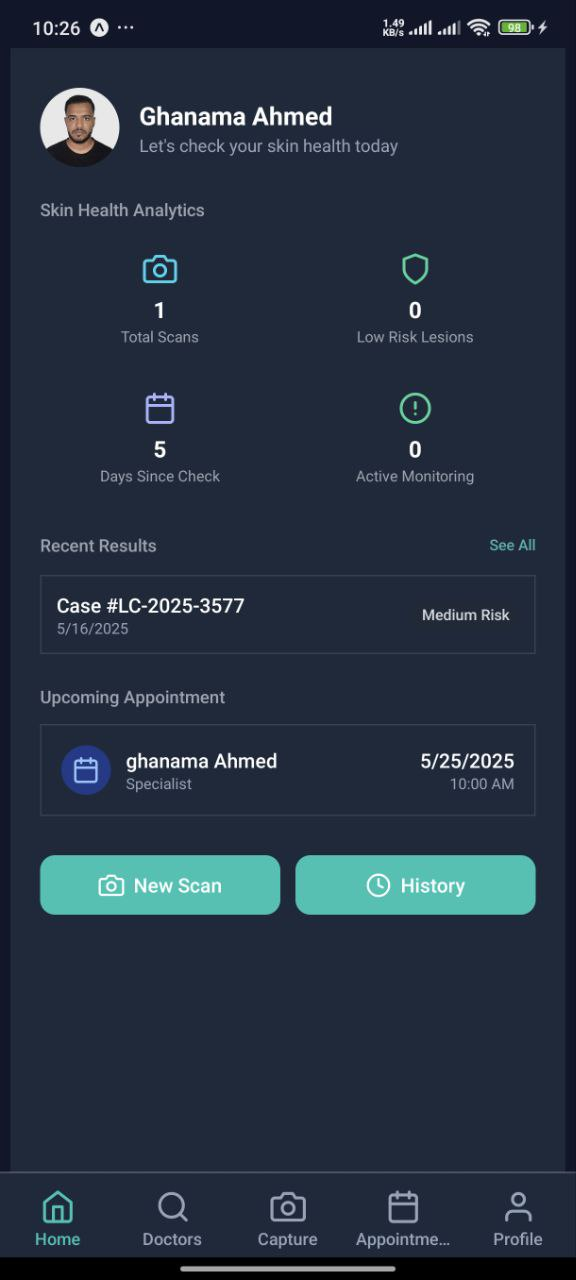
\includegraphics[width=0.5\textwidth]{photo_2_2025-06-01_09-48-58.jpg}
    \caption{DermoSxpert - Main Platform Interface / Homepage}
    \label{fig:ui_main}
\end{figure}




\begin{figure}[H]
    \centering
    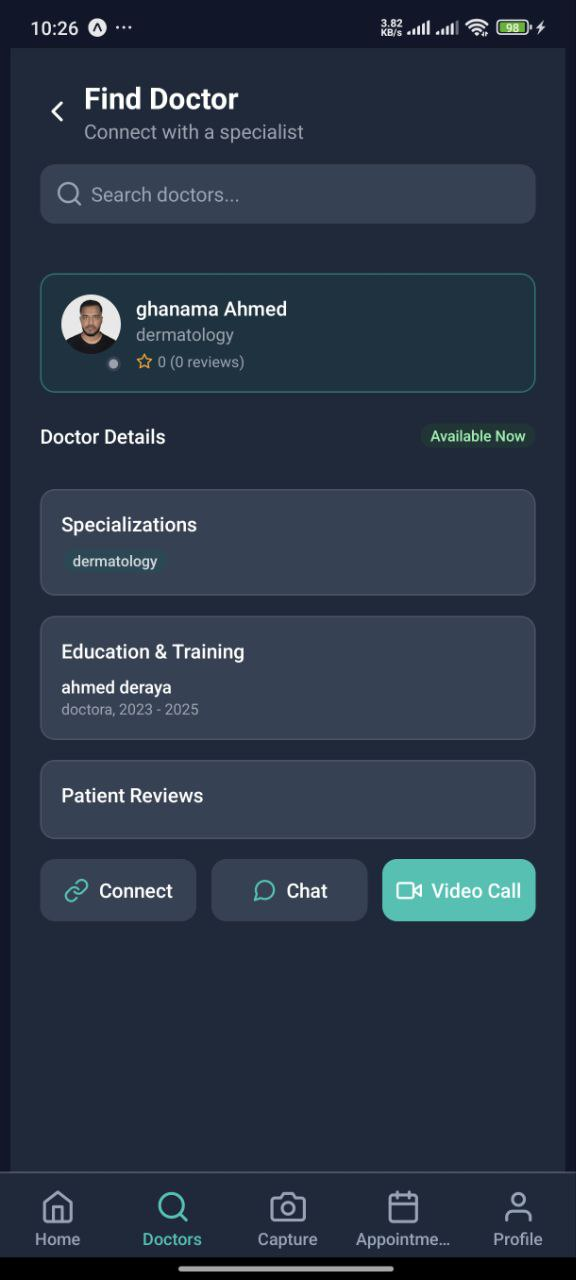
\includegraphics[width=0.5\textwidth]{photo_6_2025-06-01_09-48-58.jpg}
    \caption{DermoSxpert - Service Selection Interface (e.g., Find a Doctor, AI Skin Check)}
    \label{fig:ui_service_selection}
\end{figure}

\begin{figure}[H]
    \centering
    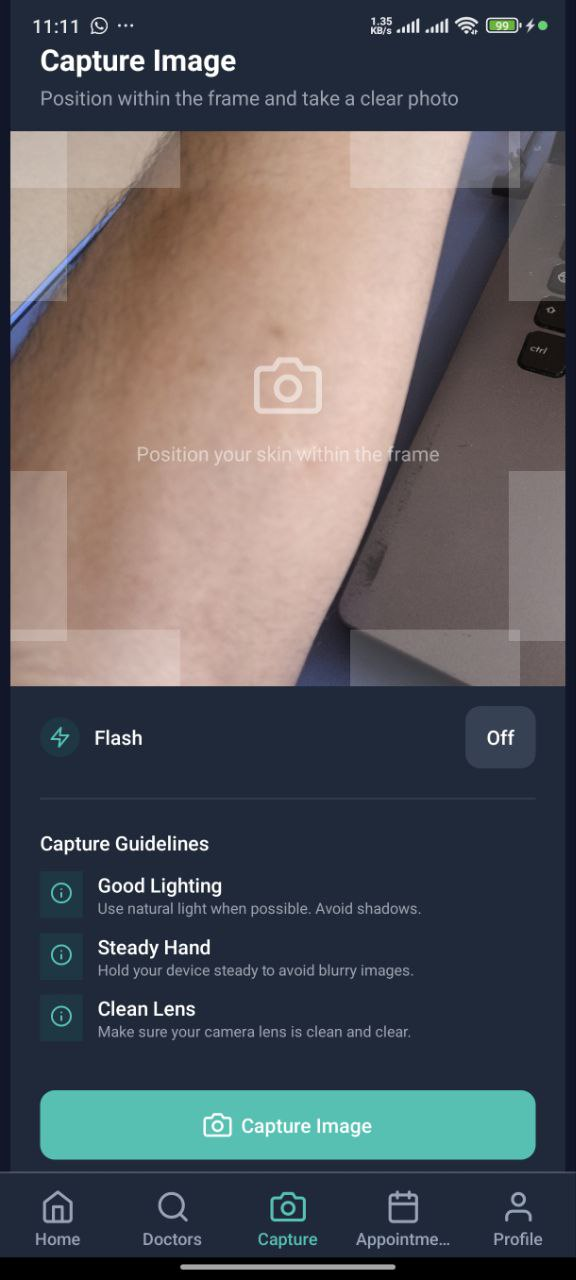
\includegraphics[width=0.5\textwidth]{photo_1_2025-06-01_09-48-58.jpg}
    \caption{DermoSxpert - AI Skin Cancer Detection Tool Interface (Capture Image)}
    \label{fig:ui_ai_tool}
\end{figure}

\begin{figure}[H]
    \centering
    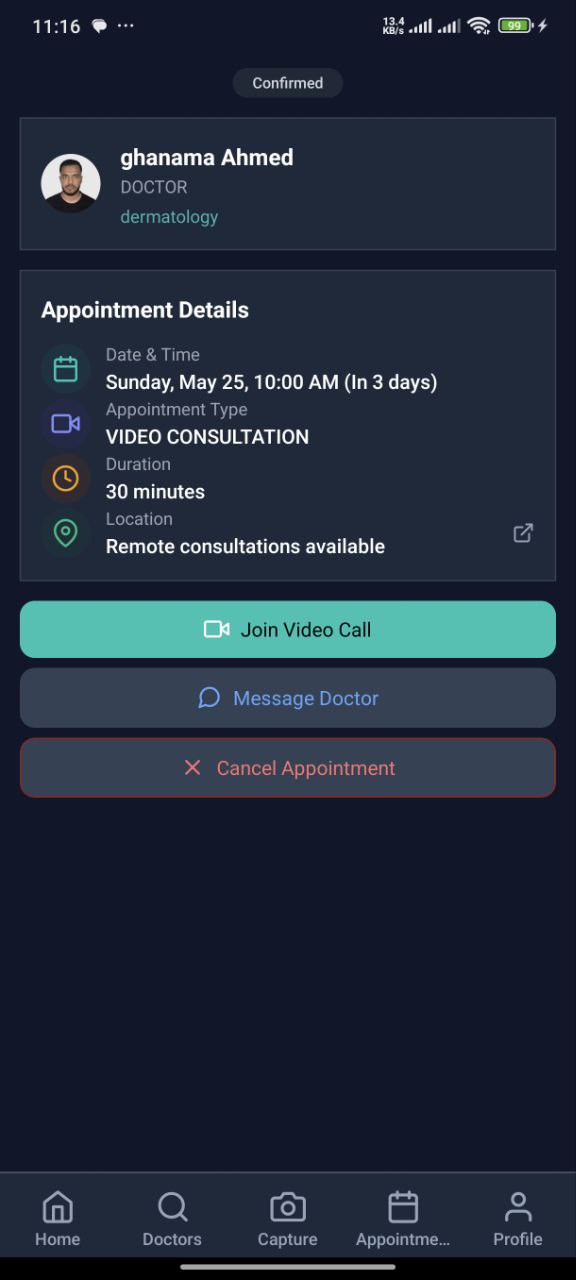
\includegraphics[width=0.5\textwidth]{photo_7_2025-06-01_09-48-58.jpg}
    \caption{DermoSxpert - Doctor's Dashboard / Consultation Interface (Appointment Details)}
    \label{fig:ui_doctor_dashboard}
\end{figure}

\begin{figure}[H]
    \centering
    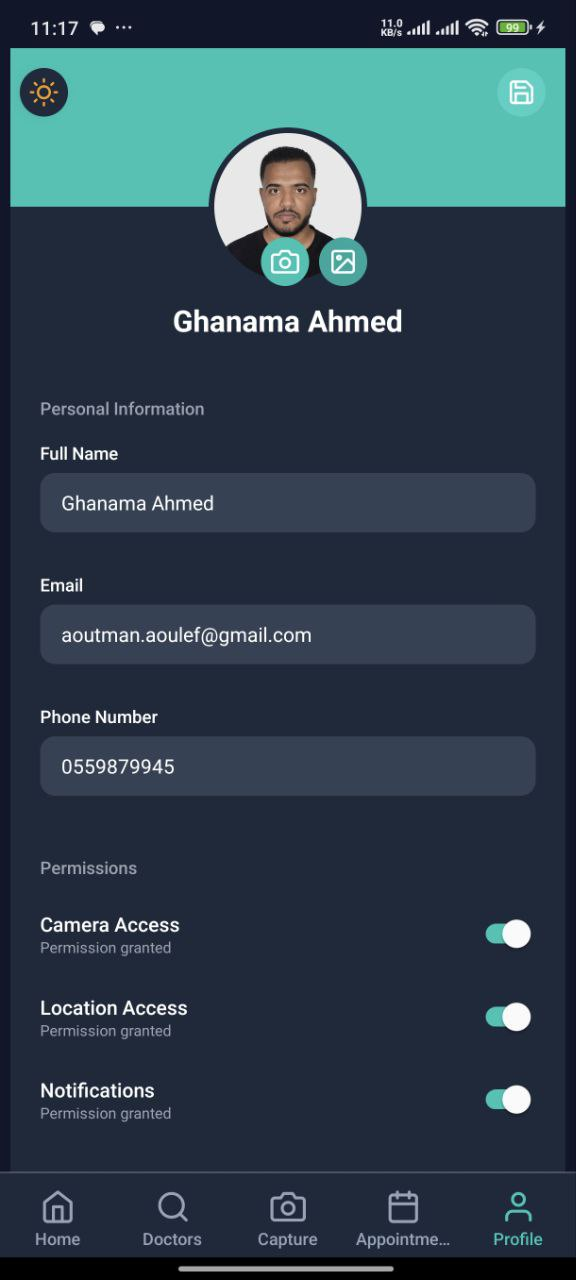
\includegraphics[width=0.5\textwidth]{photo_9_2025-06-01_09-48-58.jpg}
    \caption{DermoSxpert - About the Platform / Information Page (Profile/Personal Information)}
    \label{fig:ui_about}
\end{figure}
% Add more figures as needed for other key UI elements.


\clearpage
\thispagestyle{empty}




\end{document}
